\chapter{Marco Teórico}
\label{gb}

\section{Game Boy}
La \textbf{Game Boy} es una consola portátil de \textbf{8 bits} desarrollada y fabricada por Nintendo, lanzada al mercado el \textbf{21 de abril de 1989 en Japón}, tres meses después en América y el 28 de septiembre de 1990 en Europa. Fue la segunda consola portátil de la compañía, sucesora de la familia Game \& Watch. \\

\begin{figure}[h]
\centering
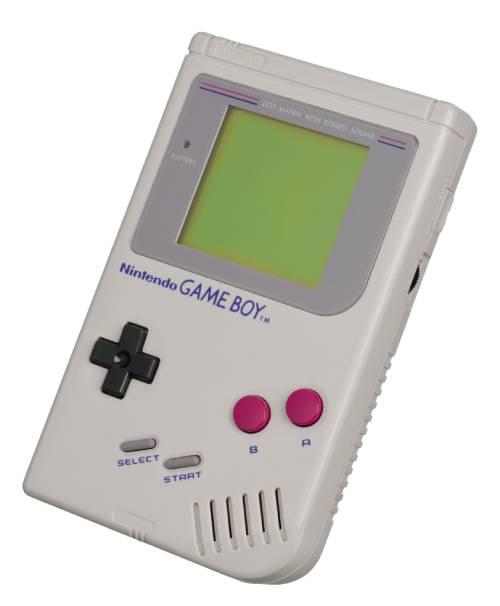
\includegraphics[width=0.15\textwidth]{include/images/gb.jpg}
\caption{Game Boy}
\label{figure:gb}
\end{figure}

Entre sus características técnicas, la Game Boy incluía un procesador Z80, una pantalla LCD monocromática con ajuste de contraste, un pad direccional de 8 direcciones, dos botones de acción (A y B) y dos botones de control (Start y Select).
\\\\
A pesar de recibir críticas por el tamaño de su pantalla y su limitada paleta de colores, la Game Boy logró un rotundo éxito comercial. Su éxito se atribuye principalmente a su bajo consumo energético, ya que funcionaba con cuatro pilas AA que ofrecían una gran autonomía en comparación con consolas rivales, como la Game Gear de SEGA. Además, la consola fue lanzada junto al exitoso juego Tetris, lo que contribuyó a su popularidad tanto entre niños como entre adultos.
\\\\
La longevidad de la Game Boy en el mercado se debe en gran parte al modelo de negocio que Nintendo continúa aplicando hoy en día, basado en la introducción de revisiones compatibles con versiones anteriores en lugar de lanzar consolas completamente nuevas. Entre estas revisiones destacan la Game Boy Pocket en 1996, así como la Game Boy Light y la Game Boy Color en 1998.

\begin{figure}[H]
\centering
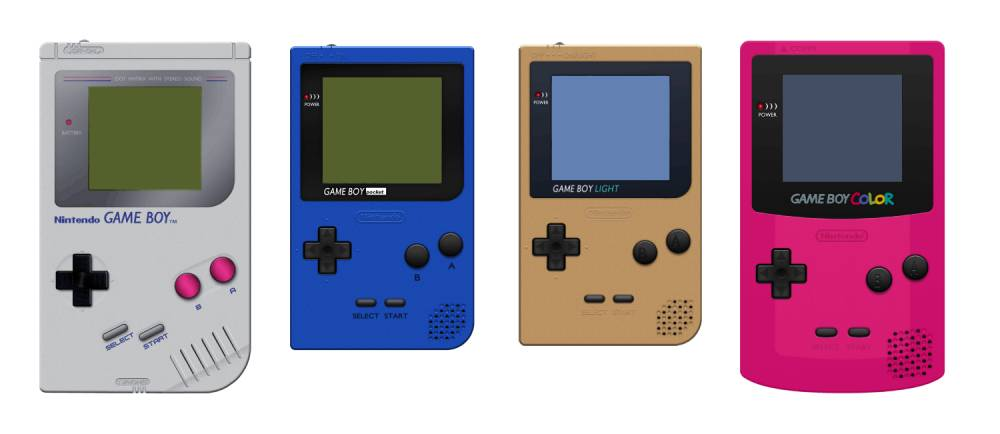
\includegraphics[width=0.7\textwidth]{include/images/gbs.jpg}
\caption{Versiones DMG, MGB, GBL y CGB de Game Boy}
\label{figure:v_gameboy}
\end{figure}

\subsection{Especificaciones Técnicas}

Cuando pensamos en programar un emulador que simule una máquina en concreto lo primero que debemos hacer es conocer exáctamente \textbf{cómo es por dentro y cómo funciona}. En la siguiente tabla quedan reflejadas todas las \textbf{características técnicas de la Game Boy}: \\

\begin{longtable}{|m{3cm}|m{2.5cm}|m{3cm}|m{2.5cm}|m{2.5cm}|}
\hline
\textbf{Características} & \textbf{Game Boy (DMG)} & \textbf{Game Boy Pocket (MGB)} & \textbf{Super Game Boy (SGB)} & \textbf{Game Boy Color (CGB)} \\
\hline
\endfirsthead
\multicolumn{5}{c}%
{\tablename\ \thetable\ -- \textit{Continúa de la página anterior}} \\
\hline
\textbf{Características} & \textbf{Game Boy (DMG)} & \textbf{Game Boy Pocket (MGB)} & \textbf{Super Game Boy (SGB)} & \textbf{Game Boy Color (CGB)} \\
\hline
\endhead
\hline \multicolumn{5}{|r|}{\textit{Continúa en la siguiente página}} \\
\endfoot
\hline
\endlastfoot

\textbf{CPU} & \multicolumn{4}{c|}{8-bit 8080-like Sharp CPU (speculated to be a SM83 core)}  \\
\hline
\textbf{Frecuencia CPU} & \multicolumn{2}{c|}{4.194304 MHz} & Depende de la revisión & Hasta 8.388608 MHz \\
\hline
\textbf{Work RAM} & \multicolumn{3}{c|}{8 KiB} & 32 KiB (4 + 7 × 4 KiB)  \\
\hline
\textbf{Video RAM} & \multicolumn{3}{c|}{8 KiB} & 16 KiB (2 × 8 KiB) \\
\hline
\textbf{Pantalla} & LCD 4.7 × 4.3 cm & LCD 4.8 × 4.4 cm & CRT TV & TFT 4.4 × 4 cm \\
\hline
\textbf{Resolución} & \multicolumn{2}{c|}{160 × 144} & 160 × 144 dentro de 256 × 224 border & 160 × 144 \\
\hline
\textbf{Sprites (OBJ)} & \multicolumn{4}{c|}{8×8 o 8×16; máximo 40 por pantalla, 10 por línea} \\
\hline
\textbf{Paletas} & \multicolumn{2}{c|}{BG: 1 × 4, OBJ: 2 × 3} & BG/OBJ: 1 + 4 × 3, border: 4 × 15 & BG: 8 × 4, OBJ: 8 × 33 \\
\hline
\textbf{Colores} & 4 tonos de verde & 4 tonos de gris & \multicolumn{2}{c|}{32768 colores (15-bit RGB)} \\
\hline
\textbf{Sincronización horizontal} & \multicolumn{2}{c|}{9.198 KHz} & Complicado\footnotemark[1] & 9.198 KHz \\
\hline
\textbf{Sincronización vertical} & \multicolumn{2}{c|}{59.73 Hz} & Complicado\footnotemark[1] & 59.73 Hz \\
\hline
\textbf{Sonido} & \multicolumn{2}{p{5cm}|}{4 canales con salida estéreo} & 4 canales GB + audio SNES & 4 canales con salida estéreo \\
\hline
\textbf{Energía} & DC 6V, 0.7 W & DC 3V, 0.7 W & Alimentado por SNES & DC 3V, 0.6 W \\
\hline

\caption{Especificaciones técnicas de la Game Boy.}
\label{table:1}
\end{longtable}

\footnotetext[1]{La SGB ejecuta dos consolas de forma simultánea: la Game Boy dentro del cartucho y la SNES. La SNES captura y muestra los gráficos de la Game Boy, pero las velocidades de fotogramas de ambas no se sincronizan completamente, lo que provoca duplicados y/o eliminados}

\subsection{Mapa de Memoria}

La Game Boy dispone de 64 Kb de memoria y utiliza direcciones de memoria de 16 bits, lo que le da la posibilidad de utilizar el rango de 0x0000 hasta 0xFFFF (65.535 bytes en total). Además, esta memoria se organiza en diferentes áreas para que el procesador pueda acceder a recursos clave como el código del juego, la memoria de video, la RAM y los registros de control. Cada una de estas áreas tiene una función específica, y algunas de ellas están sujetas a restricciones o condiciones de acceso durante la ejecución del sistema.

\begin{table}[h]
\centering
\begin{tabular}{|c|c|c|}
\hline
\textbf{Inicio} & \textbf{Fin} & \textbf{Descripción} \\ \hline
0000 & 3FFF & 16 KiB Banco ROM 00 \\ \hline
4000 & 7FFF & 16 KiB Banco ROM 01–NN \\ \hline
8000 & 9FFF & 8 KiB RAM de Vídeo (VRAM) \\ \hline
A000 & BFFF & 8 KiB RAM Externa \\ \hline
C000 & CFFF & 4 KiB Work RAM (WRAM) \\ \hline
D000 & DFFF & 4 KiB Work RAM (WRAM) \\ \hline
E000 & FDFF & Echo RAM (espejo de C000–DDFF) \\ \hline
FE00 & FE9F & Memoria de atributos de objetos (OAM) \\ \hline
FEA0 & FEFF & No usable \\ \hline
FF00 & FF7F & Registros de entrada/salida (I/O) \\ \hline
FF80 & FFFE & High RAM (HRAM) \\ \hline
FFFF & FFFF & Registro de habilitación de interrupciones (IE) \\ \hline
\end{tabular}
\caption{Mapa de memoria de Game Boy}
\end{table}

\subsubsection{ROM: [0x0000 - 0x7FFF]}
En las primeras direcciones del mapa de memoria (0x0000–0x7FFF) se encuentran los bancos de memoria ROM, que almacenan el código del juego cargado desde el cartucho. La sección entre 0x0000 y 0x3FFF es el banco fijo de 16 KiB que se carga automáticamente al encender la consola. Por último, la sección entre 0x4000 y 0x7FFF corresponde a bancos de ROM adicionales que pueden ser intercambiados (si el tipo de cartucho lo permite) para ofrecer acceso a más de 32 KiB de memoria.

\subsubsection{VRAM: [0x8000 - 0x9FFF]}\label{mem:vram}
La VRAM es una memoria de 8 KiB que se utiliza para almacenar datos gráficos, como los sprites y tiles que se dibujan en pantalla. En los modelos CGB, esta sección de la memoria tiene dos bancos, con la posibilidad de intercambiarlos entre ellos y almacenar gráficos adicionales.
\\\\
Se divide en tres secciones:
\begin{itemize}
    \item \label{mem:vram_1} \textbf{0x8000 - 0x97FF}: Bloque de memoria en el que se almacena la información de los tiles. Cada tile ocupa 16 bytes, por lo que forma general accederemos a la información de cada uno multiplicando su índice por 16 (el tile 0 hará referencia a la posición 0x8000, y el tile 1 a la posición 0x8010).
    \item \textbf{0x9800 - 0x9BFF}: Bloque de memoria de 1024 bytes en el que se almacena la información de los mapas de fondo (Background y Window). La información guardada deberán ser los índices de los tiles a dibujar.
    \item \textbf{0x9C00 - 0x9FFF}: Espejo de la sección anterior, que se utiliza para almacenar la información de los mapas de fondo en caso de que se necesite más memoria.
\end{itemize}

\begin{figure}[H]
    \centering
    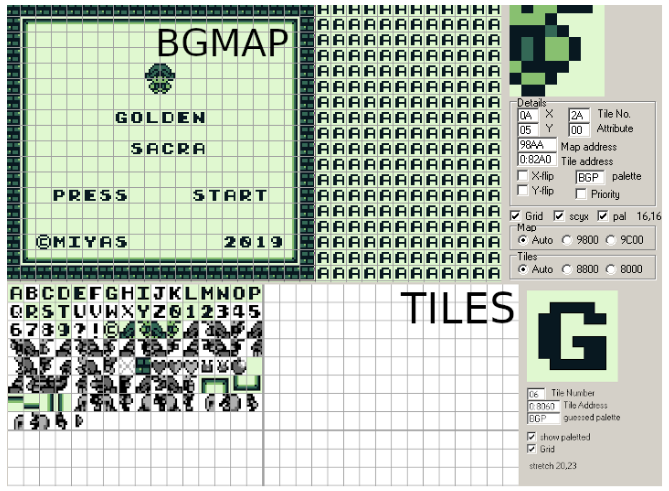
\includegraphics[width=0.8\textwidth]{include/images/mem_vram.png}
    \caption{Visualización de la memoria VRAM (\cite{goldensacra})}
    \label{figure:mem_vram}
\end{figure}

\subsubsection{RAM Externa: [0xA000 - 0xBFFF]}
Algunos cartuchos incluyen RAM adicional que se usa principalmente para guardar datos o estados del juego, como partidas guardadas. Esta RAM externa, que varía en tamaño según el cartucho, se puede acceder a través de esta región de memoria.

\subsubsection{Work RAM: [0xC000 - 0xDFFF]}
La WRAM es un área de memoria utilizada por el sistema para almacenar variables temporales, datos en proceso, y otra información necesaria para la ejecución de los programas. Está dividida en dos secciones de 4 KiB cada una. En los modelos CGB, la segunda parte (0xD000–0xDFFF) también puede ser conmutada entre diferentes bancos para aumentar la capacidad de almacenamiento.

\subsubsection{Echo RAM: [0xE000 - 0xFDFF]}
Esta es una copia exacta de la WRAM en las direcciones 0xC000–0xDDFF. Aunque se puede acceder a ella de la misma forma que la RAM original, Nintendo prohíbe su uso, ya que podría causar errores de sincronización o conflictos de acceso.

\subsubsection{OAM: [0xFE00 - 0xFE9F]}\label{mem:oam}
La OAM es un pequeño bloque de memoria dedicado a almacenar información sobre los sprites que aparecen en pantalla, como su posición, prioridad y patrones de color. Puede contener hasta un total de 40 sprites, cada uno de 8x8 u 8x16 píxeles. Sin embargo, por limitaciones de hardware, solamente se pueden mostrar 10 sprites por scanline.
\\\\
En la siguiente figura, se muestra cómo se guardarían los tiles 4 y 6 en memoria para que en pantalla se muestren de manera continua:

\begin{figure}[H]
    \centering
    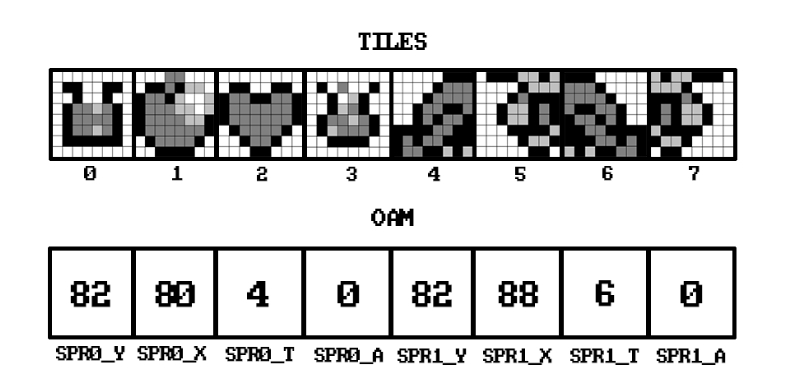
\includegraphics[width=0.6\textwidth]{include/images/oam_tiles.png}
    \caption{Datos de tiles en OAM (\cite{goldensacra})}
    \label{figure:oam_tiles}
\end{figure}

A continuación se describen los datos de forma más específica:

\begin{itemize}
    \item \textbf{Byte 0 - Posición Y}, el cual tiene un offset de 16 píxeles. Y = 0 dejaría el sprite escondido, mientras que Y = 16 lo mostraría en la parte superior de pantalla.
    
    \begin{figure}[H]
        \centering
        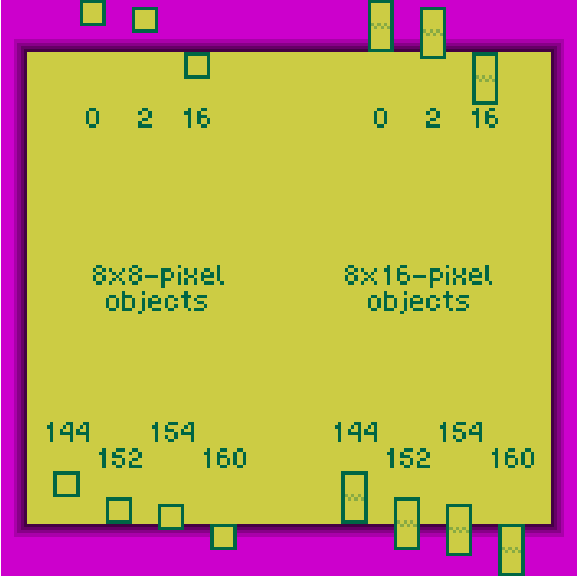
\includegraphics[width=0.5\textwidth]{include/images/y_position.png}
        \caption{Posiciones Y de los sprites (\cite{newpandocs})}
        \label{figure:y_positions}
    \end{figure}

    \item \textbf{Byte 1 - Posición X}, el cual tiene un offset de 8 píxeles.
    \item \textbf{Byte 2 - Índice de tile}. En el modo 8x8, este byte especifica un índice único de tile, dentro del rango [0x00-0xFF]. La consola selecciona internamente el tile en la VRAM, dentro de la región de memoria \hyperref[mem:vram_1]{0x8000 - 0x97FF}. En el modo 8x16, este índice corresponde al tile superior del objeto, y la consola utiliza el tile contiguo en memoria para el tile inferior, ajustando automáticamente la referencia en memoria. En modo CGB el índice se puede referir a los bancos 0 o 1 de VRAM, dependiendo del bit 3 del byte 3.
    \item \textbf{Byte 3 - Atributos}. Aplican ciertos efectos o ajustes al sprite:
        \begin{itemize}
            \item \textbf{Bit 7:} Control de la prioridad del sprite. Si su valor es 1, los tiles de Background y Window cuyos índices de color vayan del 1 al 3 se renderizarán por encima del objeto.
            \item \textbf{Bit 6:} Flip Y del sprite.
            \item \textbf{Bit 5:} Flip X del sprite.
            \item \textbf{Bit 4:} Selecciona la paleta de color para modo DMG. 0 = OBP0, 1 = OBP1.
            \item \textbf{Bit 3:} Para modos CGB, selecciona el banco de VRAM a utilizar.
            \item \textbf{Bit 2-0:} Selecciona la paleta de color para modo CGB. Va de OBP0 hasta OBP7.
        \end{itemize}

\end{itemize}

\paragraph{DMA - 0xFF46:} Mecanismo que permite la transferencia eficiente de datos desde la memoria ROM o RAM hacia la memoria OAM sin la intervención directa de la CPU. En lugar de copiar los datos byte a byte mediante instrucciones de la CPU, un controlador dedicado se encarga de mover grandes bloques de datos de manera optimizada.
\\\\
Para iniciar una transferencia DMA, se debe escribir cualquier valor en el registro 0xFF46. El valor insertado se interpretará como la parte alta de la dirección de origen y se multiplicará por 0x100. Por ejemplo, si se escribe 0x80, la transferencia comenzará desde 0x8000, mientras que si se introduce 0xC2, se iniciará desde 0xC200.
\\\\
Este proceso copia un total de \textbf{160 bytes} y requiere \textbf{160 ciclos de máquina}. En el modo \textit{CGB Double Speed}, este tiempo se reduce a la mitad. Durante la transferencia, la \textbf{CPU queda inactiva y no puede ejecutar código alojado en ROM}, ya que solo mantiene acceso a la \textbf{HRAM} (0xFF80 - 0xFFFE).


\subsubsection{No utilizable: [0xFEA0 - 0xFEFF]}
Esta pequeña área de memoria no se utiliza y está reservada. Cualquier intento de leer o escribir en esta región puede provocar comportamientos inesperados en el sistema.
\\\\
Si se intenta acceder a la región, devolverá un valor 0xFF cuando el OAM está bloqueado, y de lo contrario, dependerá de la revisión del hardware:

\begin{itemize}
    \item En DMG, MGB, SGB y SGB2, las lecturas durante el bloqueo de OAM provocan corrupción de OAM. De otra forma devolverán 0x00.
    \item En la revisión E de CGB, y los modelos AGB, AGS y GBP, devuelve el nibble alto del byte de la dirección inferior dos veces; por ejemplo, 0xFFA0 devuelve 0xAA, 0xFFB1 devuelve 0xBB, y así sucesivamente.
    \item En el resto de revisiones de CGB (0-D), la región es una sección de RAM única, pero enmascarada con un valor específico.
\end{itemize}

\subsubsection{I/O: [0xFEA0 - 0xFEFF]}
Estos registros se utilizan para controlar diferentes aspectos del hardware de la Game Boy, como la pantalla, los botones de entrada, el sonido y otros componentes del sistema. Acceder a estos registros permite al software interactuar directamente con el hardware.

\subsubsection{HRAM: [0xFF80 - 0xFFFE]}
La HRAM es un pequeño bloque de memoria de alta velocidad que contiene datos críticos que el procesador necesita acceder de manera rápida y frecuente.

\subsubsection{IE: 0xFFFF}
Registro de habilitación de interrupciones (Interrupt Enable), que permite activar o desactivar interrupciones específicas del sistema, cruciales para el manejo de eventos como temporizadores o actualizaciones gráficas.

\section{CPU}

También conocida como la Unidad Central de Procesamiento, que constituye el núcleo principal del sistema. Es la encargada de ejecutar los opcodes, que definen el comportamiento del software en la consola original.

\subsection{Diferencias}

LA Game Boy cuenta con un procesador único conocido como Sharp LR35902 y, como viene indicado en su nombre, fue desarrollado por la empresa Sharp Corporation. Esta CPU era una mezcla entre la conocida Zilog Z80 y el Intel 8080, a la cual se añadieron y eliminaron distintas instrucciones. Una diferencia importante, es que la Sharp no tiene instrucciones propias de I/O, a diferencia de las otras dos. En este caso, se puede acceder a los puertos de entrada/salida mediante comandos simples de carga (LD).
\\\\
A continuación se muestra una tabla con las diferencias existentes en el abanico de instrucciones:

\begin{table}[H]
    \centering
    \begin{tabular}{|c|c|c|}
        \hline
        \textbf{Opcode} & \textbf{Z80} & \textbf{Sharp LR35902} \\
        \hline
        08 & EX AF,AF & LD (nn),SP \\ \hline
        10 & DJNZ PC+dd & STOP \\ \hline
        22 & LD (nn),HL & LDI (HL),A \\ \hline
        2A & LD HL,(nn) & LDI A,(HL) \\ \hline
        32 & LD (nn),A & LDD (HL),A \\ \hline
        3A & LD A,(nn) & LDD A,(HL) \\ \hline
        D3 & OUT (n),A & - \\ \hline
        D9 & EXX & RETI \\ \hline
        DB & IN A,(n) & - \\ \hline
        DD & \textless IX\textgreater prefix & - \\ \hline
        E0 & RET PO & LD (FF00+n),A \\ \hline
        E2 & JP PO,nn & LD (FF00+C),A \\ \hline
        E3 & EX (SP),HL & - \\ \hline
        E4 & CALL P0,nn & - \\ \hline
        E8 & RET PE & ADD SP,dd \\ \hline
        EA & JP PE,nn & LD (nn),A \\ \hline
        EB & EX DE,HL & - \\ \hline
        EC & CALL PE,nn & - \\ \hline
        ED & \textless prefix\textgreater & - \\ \hline
        F0 & RET P & LD A,(FF00+n) \\ \hline
        F2 & JP P,nn & LD A,(FF00+C) \\ \hline
        F4 & CALL P,nn & - \\ \hline
        F8 & RET M & LD HL,SP+dd \\ \hline
        FA & JP M,nn & LD A,(nn) \\ \hline
        FC & CALL M,nn & - \\ \hline
        FD & \textless IY\textgreater prefix & - \\ \hline
        CB 3X & SLL r/(HL) & SWAP r/(HL) \\
        \hline
    \end{tabular}
    \caption{Comparación de opcodes entre Z80 y Sharp LR35902}
\end{table}

Los opcodes que se indican con un "-" significan que han sido eliminados. Si intentáramos utilizar los originales, la Game Boy simplemente se congelaría y habría que reiniciar el sistema.

\subsection{Registros}

Un registro es una pequeña unidad de almacenamiento en un procesador utilizada para guardar temporalmente datos o instrucciones durante la ejecución de operaciones. Los registros que se emplean son: A, F, B, C, D, E, H y L, cada uno capaz de almacenar 1 byte de información. Estos registros también pueden agruparse en pares para manejar 2 bytes: AF, BC, DE y HL. Adicionalmente, los registros SP (Stack Pointer) y PC (Program Counter) desempeñan funciones específicas dentro de la CPU.
\\\\
El primer registro a destacar es el registro A, conocido como el Acumulador, donde se almacena la mayoría de los datos procesados por la CPU. Es un registro al que se le pueden asignar valores de forma directa, al igual que ocurre con los registros B, C, D, E, H y L.
\\\\
Los registros B y C son comúnmente utilizados como contadores, mientras que los registros D y E se suelen emplear en pares para almacenar direcciones de memoria, facilitando operaciones de copia de datos. Sin embargo, el uso de estos registros no está limitado a estos propósitos; su aplicación depende de las necesidades y la conveniencia del programador.
\\\\
El registro F o Flags es responsable de almacenar el estado actual del procesador, y es de solo lectura. Aunque no se puede modificar directamente, su combinación con el registro A es clave para realizar diversas operaciones. Su principal utilidad radica en la evaluación de los resultados de la instrucción anterior, siendo esencial para la toma de decisiones en la ejecución del programa.
\\\\
En la siguiente tabla podemos ver el desglose del valor atribuido a cada bit del registro F:

\begin{table}[H]
    \centering
    \begin{tabular}{|c|c|>{\centering\arraybackslash}p{9cm}|}
        \hline
        \textbf{Bit} & \textbf{Nombre} & \textbf{Definición} \\
        \hline
        7 & Z & Zero: indica si el resultado de la operación previa ha dado como resultado 0. \\
        \hline
        6 & N & Substraction: indica si la operación previa ha sido una resta. \\
        \hline
        5 & H & Semi-Carry: indica si se ha producido un acarreo desde el nibble bajo al alto en la operación de suma o resta anterior. \\
        \hline
        4 & C o CY & Carry: indica si se ha producido un acarreo en el bit más significativo, es decir, el resultado ha sido mayor de 0xFF. \\
        \hline
        3-0 & - & No se utilizan. \\
        \hline
    \end{tabular}
    \caption{Función de los bits del registro F o Flags}
\end{table}

Por su parte, los registros H y L se utilizan para el acceso indirecto a una dirección de memoria. Este acceso indirecto se refiere al valor de 16 bits contenido en la pareja de registros HL, y resulta especialmente útil para recorrer arrays o acceder secuencialmente a posiciones de memoria.
\\\\
El registro SP (Stack Pointer) señala la posición de memoria que se utiliza durante las llamadas a subrutinas. Al ejecutar una instrucción call, la pila aumenta, y al realizar un ret, la pila disminuye, permitiendo mantener el control del flujo de ejecución.
\\\\
Finalmente, el registro PC (Program Counter) indica la dirección de memoria donde se encuentra la próxima instrucción que será ejecutada por la CPU, siendo esencial para el flujo de control del programa.

\subsection{Opcodes}

Los opcodes (códigos de operación) son las instrucciones que un procesador entiende y ejecuta directamente. Representan la parte de una instrucción de máquina que especifica la operación a realizar, como cargar datos en un registro, realizar una operación matemática o mover datos entre la memoria y el procesador. Cada opcode tiene un formato específico y puede estar compuesto por varios bytes que definen tanto la operación como los operandos involucrados.

\subsubsection{Categorías}

En total, existen 510 instrucciones diferentes, las cuales pueden ser agrupadas en las siguientes categorías:
\begin{itemize}
  \item \textbf{Operaciones de carga (LD)}
  \begin{itemize}
  \item LD A, (HL): Carga el valor de la dirección de memoria en el registro A.
  \item LD (HL), B: Carga el valor del registro B en la memoria apuntada por HL.
  \end{itemize}
  \item \textbf{Operaciones aritméticas y lógicas}
  \begin{itemize}
  \item ADD A, B: Suma el contenido de B al registro A.
  \item AND A: Realiza una operación lógica AND en el registro A.
  \item SUB A, B: Resta el valor de B del registro A.
  \item XOR A: Realiza una operación XOR entre el registro A consigo mismo, lo que siempre da como resultado 0. Este comando se utiliza para limpiar o reiniciar el registro A.
  \item OR A: Realiza una operación OR del registro A consigo mismo, dejando el valor de A sin cambios. No afecta el valor, pero puede modificar los flags.
  \item CP A: Compara el valor del registro A con el valor de otro registro o inmediato, estableciendo los flags según el resultado de la comparación. La operación es similar a una resta (A - valor) y no modifica el contenido de A.
  \item CPL: Complementa el valor del registro A, invirtiendo todos sus bits. Esta operación afecta el flag de medio acarreo (H) y establece el flag de negativo (N).
  \item CCF: Cambia el estado del flag de acarreo (C). Si el flag de acarreo está establecido, se limpia; si está limpio, se establece. Esta operación no afecta a los demás flags.
  \item DAA: Ajusta el contenido del registro A para que represente un valor decimal válido, teniendo en cuenta el estado de los flags de acarreo (C) y medio acarreo (H). Esta operación es útil después de realizar operaciones aritméticas en el modo BCD.
  \item SCF: Establece el flag de acarreo (C) y limpia el flag de acarreo (H). Esta operación no afecta a los demás flags y es útil para preparar operaciones que requieren un estado de acarreo conocido.
  \end{itemize}
  \item \textbf{Operaciones de control de flujo}
  \begin{itemize}
  \item JP nn: Salta a la dirección de memoria nn.
  \item CALL nn: Llama a una subrutina en la dirección nn.
  \item RET: Retorna de una subrutina.
  \end{itemize}
  \item \textbf{Operaciones de rotación y desplazamiento}
  \begin{itemize}
  \item RL A: Rota los bits del registro A hacia la izquierda a través del carry.
  \item SLA B: Desplaza los bits de B hacia la izquierda.
  \item RR A: Rota los bits del registro A hacia la derecha a través del carry, trasladando el bit menos significativo al carry y el carry al bit más significativo.
  \item RLC A: Rota los bits del registro A hacia la izquierda, desplazando el bit más significativo al carry y reiniciando el bit más significativo con el valor original del carry.
  \item RRC A: Rota los bits del registro A hacia la derecha, moviendo el bit menos significativo al carry y llenando el bit más significativo con el valor del carry.
  \item SRA B: Desplaza los bits de B hacia la derecha, manteniendo el bit más significativo (signo) constante y colocando el bit menos significativo en el carry.
  \item SWAP B: Intercambia los cuatro bits más significativos con los cuatro menos significativos del registro B.
  \item SRL B: Desplaza los bits de B hacia la derecha, moviendo el bit menos significativo al carry y rellenando el bit más significativo con 0.
  \end{itemize}
  \item \textbf{Operaciones de manipulación de bits}
  \begin{itemize}
  \item BIT 0, A: Prueba si el bit 0 de A está establecido.
  \item SET 1, (HL): Establece el bit 1 en la dirección de memoria HL.
  \item RES 0, A: Reinicia (pone a 0) el LSB del registro A, dejando los demás bits sin cambios.
  \end{itemize}
  \item \textbf{Operaciones especiales de sistema}
  \begin{itemize}
  \item NOP: No realiza ninguna operación.
  \item DI: Deshabilita interrupciones.
  \item EI: Habilita interrupciones.
  \end{itemize}
  \item \textbf{Operaciones con pila}
  \begin{itemize}
  \item PUSH BC: Empuja el contenido del registro BC en la pila.
  \item POP AF: Restaura el contenido de AF desde la pila.
  \end{itemize}
  \item \textbf{Operaciones I/O}
  \begin{itemize}
  \item LD (FF00+n), A: Carga el valor de A en la dirección de I/O FF00+n.
  \item LD A, (FF00+C): Carga el valor de la dirección FF00+C en A.
  \end{itemize}
\end{itemize}

\subsubsection{Listado}
Para poder empezar a implementar todos los opcodes, debemos hacer uso de la documentación (oficial o no) que nos indique qué Byte hace referencia a qué opcode. Las siguientes tablas suelen ser de gran ayuda para verlo de forma clara y concisa:

\begin{figure}[H]
\centering
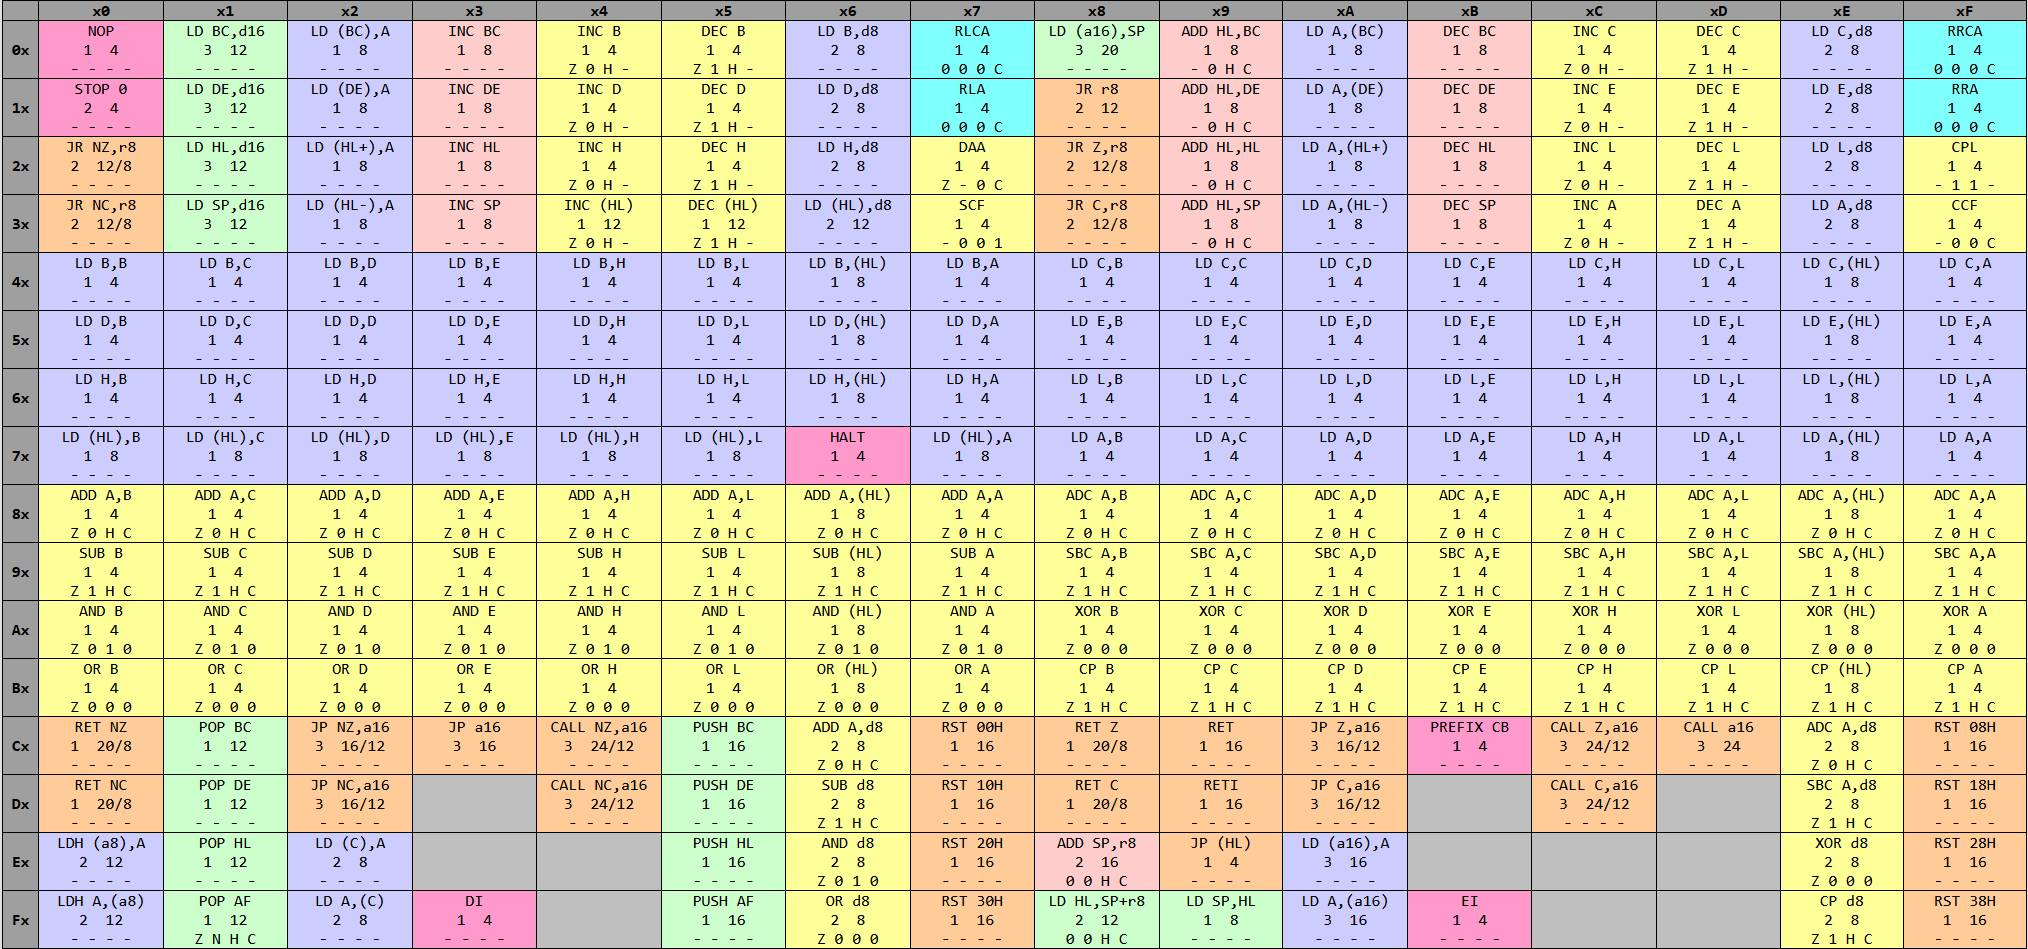
\includegraphics[width=1\textwidth]{include/images/opcodes_1.jpg}
\caption{Set de Instrucciones (\cite{opcodes})}
\label{figure:opcodes_1}
\end{figure}

\begin{figure}[H]
\centering
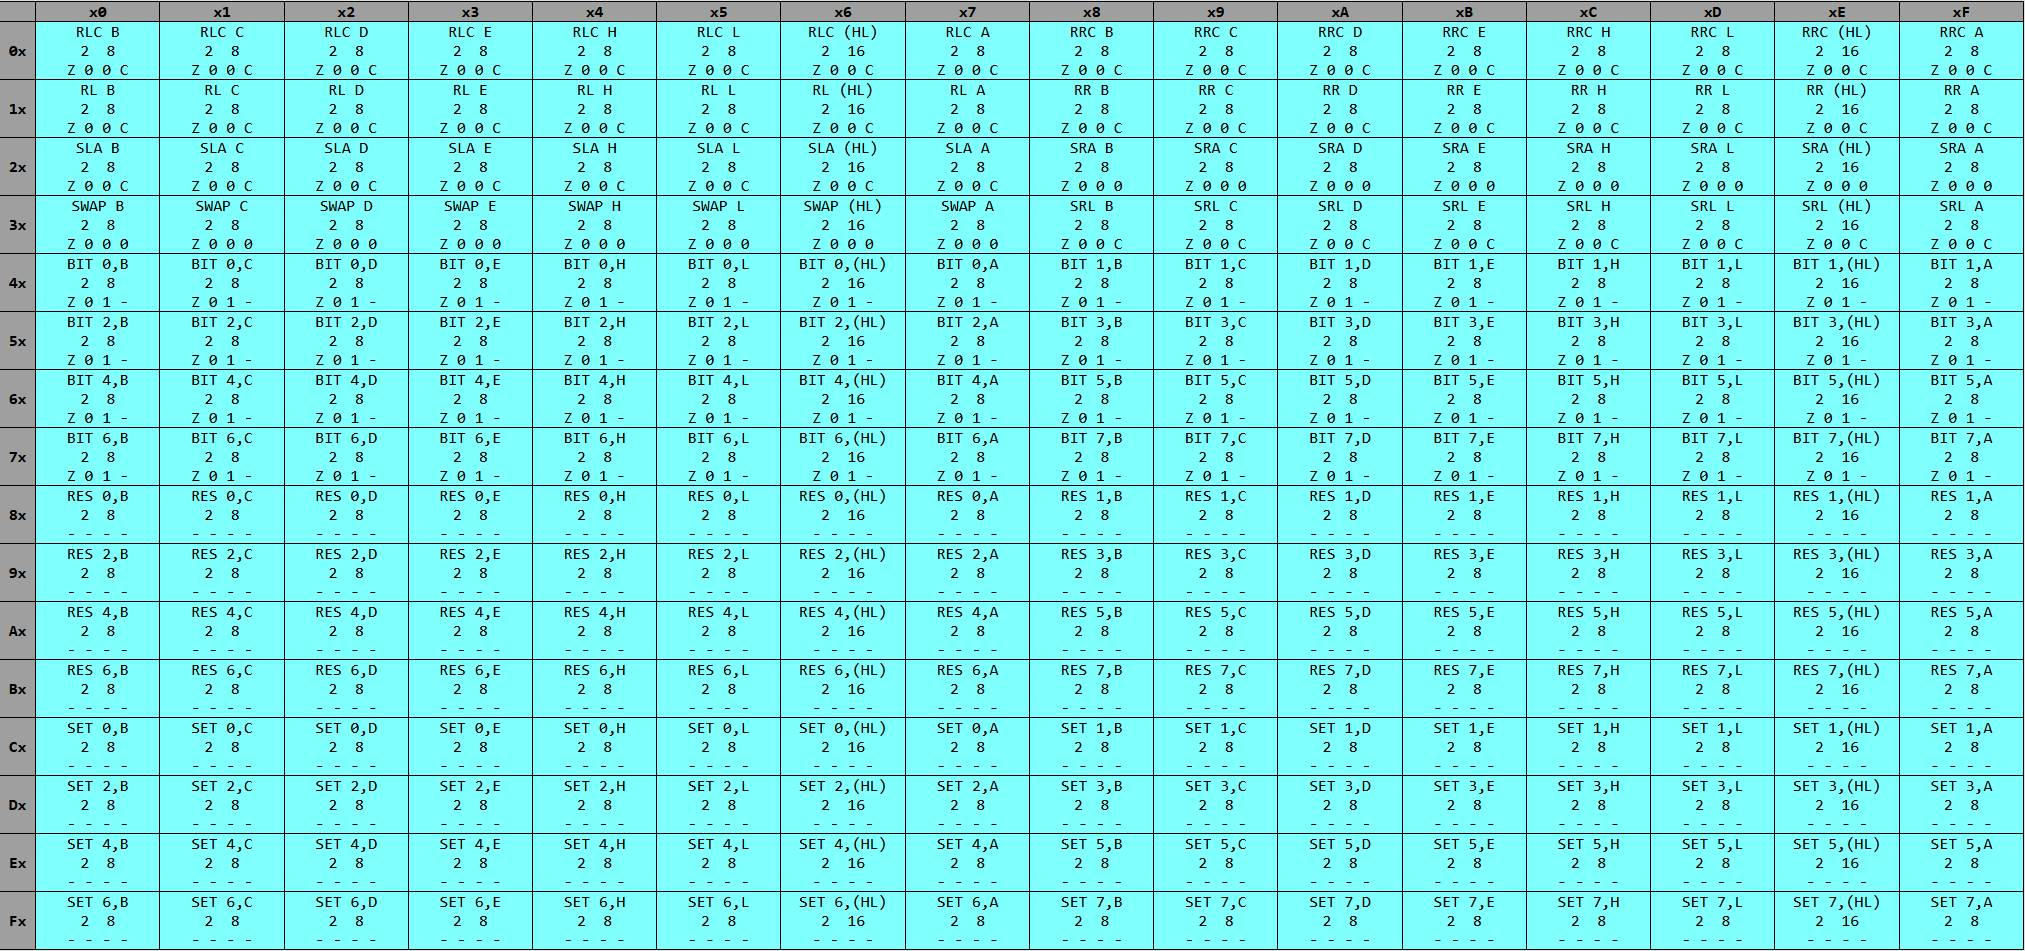
\includegraphics[width=1\textwidth]{include/images/opcodes_2.jpg}
\caption{Set de Instrucciones Extendidas (\cite{opcodes})}
\label{figure:opcodes_2}
\end{figure}

Con estas tablas obtenemos las siguientes características de cada instrucción:
\begin{itemize}
    \item \textbf{Byte} asignado.
    \item \textbf{Ciclos} de reloj.
    \item \textbf{Flags} a ignorar, actualizar o resetear.
    \item \textbf{Categoría}, agrupados por colores.
    \item \textbf{Longitud}, es decir, los bytes que la instrucción va a ocupar en memoria.
\end{itemize}

\subsection{Ciclos}

Los ciclos de CPU son unidades de tiempo en las que se realizan instrucciones. Son utilizadas para saber con exactitud cuánto tiempo dura la ejecución de una instrucción concreta en el hardware original. Hay dos conceptos distintos en este contexto: ciclos de máquina y ciclos de reloj.
\\\\
Cada componente, como la CPU, la memoria, el PPU y el APU, opera en función de los ciclos de reloj. La coordinación precisa entre estos módulos asegura que las instrucciones se ejecuten en el momento adecuado y que los datos se transfieran de manera eficiente.
\\\\
Por ejemplo, el procesador necesita esperar que el PPU complete la renderización de un cuadro antes de actualizar la pantalla, lo que implica un control cuidadoso del tiempo. Si un módulo se desincroniza, puede resultar en fallos gráficos, sonido entrecortado o un rendimiento general deficiente. Por lo tanto, la medición de ciclos de reloj permite establecer un ritmo de operación coherente, asegurando que todos los componentes funcionen armónicamente, lo que es fundamental para la experiencia de juego fluida y efectiva que caracteriza a la Game Boy.
\\\\
Para la Game Boy, 1 ciclo de máquina equivale a 4 ciclos de reloj.

\subsubsection{Ciclos de Máquina}
Los ciclos de máquina se refieren a la cantidad de ciclos de CPU necesarios para ejecutar una instrucción específica. Cada instrucción puede requerir un número diferente de ciclos de máquina, dependiendo de su complejidad.

\subsubsection{Ciclos de Reloj}
Los ciclos de reloj, por otro lado, son las unidades de tiempo que marcan el ritmo del funcionamiento del procesador. Cada ciclo de reloj representa un pulso generado por un oscilador interno en el procesador, que sincroniza las operaciones del mismo. La frecuencia del reloj, medida en hertzios (Hz), determina cuántos ciclos de reloj se producen por segundo.

\section{ROM}
\subsection{Secuencia de Arranque}

Existe una secuencia de arranque, conocido como \textbf{Boot ROM}, guardado dentro de la propia CPU. Esta secuencia de arranque comienza su ejecución en la dirección de memoria 0x000, y no en la oficial de 0x100. Este programa es responsable de la animación de arranque que se reproduce antes de que el control sea transferido a la ROM del cartucho, además de inicializar distintos registros y direcciones de memoria.
\\\\
Existen en total 9 programas de boot (conocidos hasta la fecha):
\begin{table}[h!]
\centering
\begin{tabular}{|l|c|}
\hline
\textbf{Nombre} & \textbf{Tamaño (bytes)} \\ \hline
DMG0 & 256 \\ \hline
DMG  & 256 \\ \hline
MGB  & 256 \\ \hline
SGB  & 256 \\ \hline
SGB2 & 256 \\ \hline
CGB0 & 256 + 1792 \\ \hline
CGB  & 256 + 1792 \\ \hline
AGB0 & 256 + 1792 \\ \hline
AGB  & 256 + 1792 \\ \hline
\end{tabular}
\caption{Resumen de las variaciones de las secuencias de arranque}
\end{table}

\subsubsection{DMG / MGB}
Lo primero que hacen es leer el logo desde el cartucho, descomprimirlo en VRAM y comenzar a desplazarlo lentamente hacia abajo. Dado que las lecturas de un cartucho ausente generalmente devuelven 0xFF, esto explica por qué, al encender la consola sin un cartucho, aparece un cuadro negro desplazándose. Además, conexiones defectuosas o sucias pueden hacer que los datos leídos se corrompan, lo que resulta en un logo desordenado.
\\\\
Una vez que el logo ha terminado de desplazarse, la boot ROM reproduce el famoso sonido \textit{"ba-ding!”} y vuelve a leer el logo, esta vez comparándolo con una copia almacenada en ROM. También calcula el checksum del encabezado y lo compara con el checksum almacenado en el encabezado. Si alguna de estas verificaciones falla, la boot ROM se bloquea y nunca se transfiere el control a la ROM del cartucho.
\\\\
Finalmente, la boot ROM escribe en el registro BANK en 0xFF50, lo que desasigna la boot ROM.
\\\\
Las diferencias con DMG0 (algunos primeros modelos de DMG), es que al fallar el checksum, la pantalla empieza a parpadear a la hora de bloquear la ROM, y que el logo de Nintendo no tiene el símbolo ®.

\subsubsection{CGB / AGB}
Estas secuencias de arranque son mucho más complejas, en especial por su comportamiento de retro-compatibilidad.
\\\\
La ROM de arranque es más grande. Aún debe ser mapeada comenzando en 0x0000, ya que es donde comienza la CPU, pero también debe acceder al encabezado del cartucho en 0x0100-0x014F. Por lo tanto, la ROM de arranque se divide en dos partes: una de 0x0000-0x00FF y otra de 0x0200-0x08FF.
\\\\
Primero, las ROMs de arranque descomponen el logo de Nintendo en VRAM, al igual que los modelos antiguos, y copian el logo a un búfer en HRAM al mismo tiempo.
\\\\
Luego, el logo se lee y descomprime nuevamente, pero sin redimensionamiento, lo que produce un logo mucho más pequeño colocado debajo del gran \textit{"GAME BOY"}. La ROM de arranque luego configura las paletas de compatibilidad, como se describe más adelante, y reproduce la animación del logo con el sonido de \textit{"ba-ding!"}.
\\\\
Durante la animación del logo, se permite al usuario elegir una paleta para anular la seleccionada para compatibilidad (con distintas secuencias de botones). Cada nueva elección evita que la animación termine durante 30 fotogramas, lo que retrasa el checksum y la transición final.
\\\\
Finalmente, la ROM de arranque desvanece todas las paletas de Background a blanco y establece el hardware en modo de compatibilidad (recordemos que existen juegos como Pokémon Oro/Plata que son de GBC pero se pueden jugar en DMG). En función del valor del byte de compatibilidad CGB, los valores a insertar en distintos registros de CGB variarán.

\subsection{Cabecera del Cartucho}

Todos los cartuchos de Game Boy contienen una cabecera ubicada en el rango de direcciones 0x100-0x14F. Esta cabecera contiene información esencial para el funcionamiento del juego y del sistema, permitiendo a los desarrolladores configurar diversos parámetros que describen las características del cartucho. Entre estos parámetros se incluyen el título del juego, el código de licencia, el tipo de cartucho (que define si utiliza RAM, batería, o expansión como MBC), y otros datos relevantes. A continuación, se detallan los registros presentes en este rango de direcciones:

\subsubsection{0x0100 - 0x0103: Punto de entrada}
Después de mostrar el logotipo de Nintendo, el PC salta a la dirección 0x0100, para a posterior saltar al inicio del programa del juego. La mayoría de los desarrolladores llenan esta área de 4 bytes con una instrucción NOP seguida de un JP 0x0150.

\subsubsection{0x0104 - 0x0133: Nintendo logo}
Esta área contiene una imagen en mapa de bits que se muestra cuando se enciende la consola. Debe coincidir con el siguiente volcado (en hexadecimal); de lo contrario, la ROM de arranque no permitirá que el juego se ejecute:

\begin{lstlisting}[language=Kotlin, caption={Nintendo Logo - Mapa de Bits}, label={code:nintendologobits}]
    CE ED 66 66 CC 0D 00 0B 03 73 00 83 00 0C 00 0D
    00 08 11 1F 88 89 00 0E DC CC 6E E6 DD DD D9 99
    BB BB 67 63 6E 0E EC CC DD DC 99 9F BB B9 33 3E
\end{lstlisting}

La forma en la que estos bytes se decodifican es la siguiente:
\begin{itemize}
    \item Los bytes en el rango 0x104-0x011B representan la mitad superior del logo, mientras que los del rango 0x11C-0x133 representan la mitad inferior.
    \item Por cada byte, cada nibble codifica 4 píxeles. Un pixel está encendido si su bit correspondiente tiene un valor de 1.
    \item Cada dos bytes componen un grupo, el cual representa una parte (inferior o superior) de una letra del logo.
\end{itemize}

\begin{figure}[H]
\centering
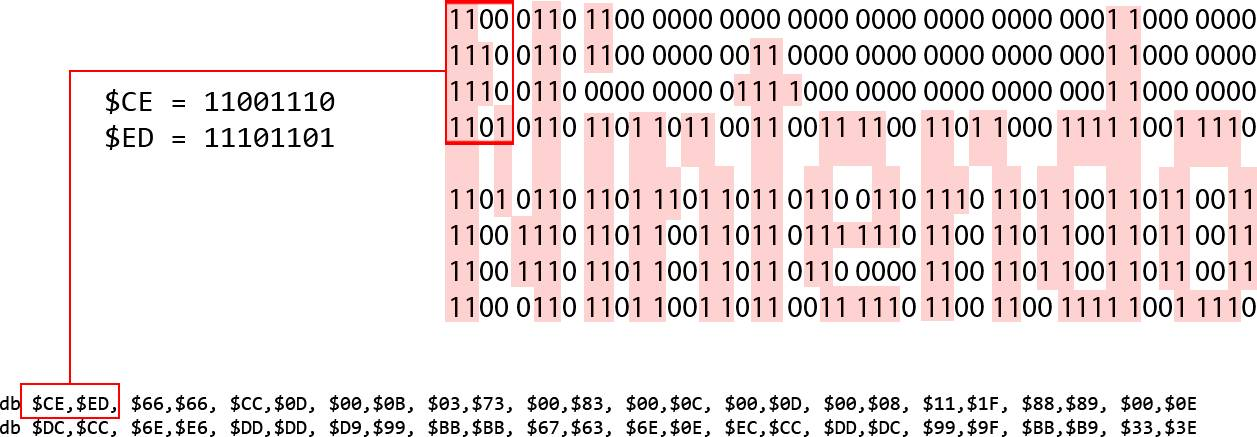
\includegraphics[width=1\textwidth]{include/images/dibujado_logo_n.jpg}
\caption{Decodificación del logo de Nintendo}
\label{figure:decodednlogo}
\end{figure}

El procedimiento de arranque de la Game Boy primero muestra el logo y luego verifica que coincida con el volcado anterior (conocido como \textit{checksum}). Si no coincide, la ROM de arranque se bloquea.
\\\\
Los modelos a partir del CGB solo verifican la mitad superior (los primeros 18 bytes).

\subsubsection{0x0134 - 0x0143: Título}
Esta región de bytes contienen el título del juego, con carácteres ASCII y completamente en mayúsculas. Si el título tiene menos de 16 carácteres, el resto de bytes deberán rellenarse con 0x00's. 
\\\\
En versiones posteriores de los cartuchos, partes de esta área tienen un significado diferente, lo que reduce el tamaño real a 15 u 11 carácteres (siempre empezando en la dirección 0x134).

\subsubsection{0x013F - 0x0142: Código de fabricante}

En los cartuchos más antiguos, estos bytes formaban parte del título. En los cartuchos más nuevos, contienen un código de fabricante de 4 caracteres (en mayúsculas ASCII). Se desconoce su propósito.

\subsubsection{0x0143: CGB Flag}
Este byte, al igual que con el código de fabricante, formaba parte del título. Los modelos CGB y posteriores lo interpretan para decidir si habilitan el modo Color ("Modo CGB") o si retroceden al modo de compatibilidad monocromático ("Modo no CGB").
\\\\
Los valores más típicos son: 
\begin{itemize}
    \item 0x00: No indicaría nada realmente, lo que implica que el juego solamente funciona en modelos DMG/MGB.
    \item 0x80: Indica que el juego admite mejoras propias del modelo CGB, pero es retro-compatible con modelos anteriores (DMG, MGB, etc...).
    \item 0xC0: El juego solamente funciona en CGB.
\end{itemize}

Valores que tengan activados los bits 7, 3 o 2, activarán un estado poco utilizado, conocido como "Modo PGB" (Pseudo Game Boy Mode). Es una especie de modo intermedio que brinda compatibilidad con juegos diseñados para el Game Boy Color cuando se ejecutan en un Game Boy original o en un Super Game Boy, pero con mejoras visuales muy limitadas en comparación con el modo CGB completo.
\\\\
Hay poca información al respecto de este modo y varias fuentes agradecen su estudio y documentación.

\subsubsection{0x0144 – 0x0145: Nuevo código de licencia}
Esta región contiene un código representado por dos carácteres ASCII, el cual indica el editor/desarrollador del juego. Solamente se utiliza en caso de que el antiguo código de licencia tenga un valor de 0x33 (suele ser el caso para los juegos publicados después de la salida de SGB).
\\\\
Los códigos son los siguientes:
\begin{longtable}{|c|l|}
\hline
\textbf{Código} & \textbf{Editor} \\ \hline
00              & Ninguno                        \\ \hline
01              & Nintendo Research \& Development 1 \\ \hline
08              & Capcom                         \\ \hline
13              & EA (Electronic Arts)           \\ \hline
18              & Hudson Soft                    \\ \hline
19              & B-AI                           \\ \hline
20              & KSS                            \\ \hline
22              & Oficina de Planificación WADA  \\ \hline
24              & PCM Complete                   \\ \hline
25              & San-X                          \\ \hline
28              & Kemco                          \\ \hline
29              & SETA Corporation               \\ \hline
30              & Viacom                         \\ \hline
31              & Nintendo                       \\ \hline
32              & Bandai                         \\ \hline
33              & Ocean Software/Acclaim Entertainment \\ \hline
34              & Konami                         \\ \hline
35              & HectorSoft                     \\ \hline
37              & Taito                          \\ \hline
38              & Hudson Soft                    \\ \hline
39              & Banpresto                      \\ \hline
41              & Ubi Soft                       \\ \hline
42              & Atlus                          \\ \hline
44              & Malibu Interactive             \\ \hline
46              & Angel                          \\ \hline
47              & Bullet-Proof Software          \\ \hline
49              & Irem                           \\ \hline
50              & Absolute                       \\ \hline
51              & Acclaim Entertainment          \\ \hline
52              & Activision                     \\ \hline
53              & Sammy USA Corporation          \\ \hline
54              & Konami                         \\ \hline
55              & Hi Tech Expressions            \\ \hline
56              & LJN                            \\ \hline
57              & Matchbox                       \\ \hline
58              & Mattel                         \\ \hline
59              & Milton Bradley Company         \\ \hline
60              & Titus Interactive              \\ \hline
61              & Virgin Games Ltd.              \\ \hline
64              & Lucasfilm Games                \\ \hline
67              & Ocean Software                 \\ \hline
69              & EA (Electronic Arts)           \\ \hline
70              & Infogrames                     \\ \hline
71              & Interplay Entertainment        \\ \hline
72              & Broderbund                     \\ \hline
73              & Sculptured Software            \\ \hline
75              & The Sales Curve Limited        \\ \hline
78              & THQ                            \\ \hline
79              & Accolade                       \\ \hline
80              & Misawa Entertainment           \\ \hline
83              & lozc                           \\ \hline
86              & Tokuma Shoten                  \\ \hline
87              & Tsukuda Original               \\ \hline
91              & Chunsoft Co.                   \\ \hline
92              & Video System                   \\ \hline
93              & Ocean Software/Acclaim Entertainment \\ \hline
95              & Varie                          \\ \hline
96              & Yonezawa/s’pal                 \\ \hline
97              & Kaneko                         \\ \hline
99              & Pack-In-Video                  \\ \hline
9H              & Bottom Up                      \\ \hline
A4              & Konami (Yu-Gi-Oh!)             \\ \hline
BL              & MTO                            \\ \hline
DK              & Kodansha                       \\ \hline
\caption{Código de licencia y su editor.} \\
\end{longtable}

\subsubsection{0x0146: SGB Flag}
Especifica si el juego es compatible con funciones del modelo SGB. El SGB ignorará cualquier transferencia de datos si el valor de este byte no es 0x03.

\subsubsection{0x0147: Tipo de cartucho}
Especifica qué tipo de hardware está presente en el cartucho (para ser más especifico, su \textit{mapper}).
\\\\
Los mappers son los siguientes:
\begin{longtable}{|c|l|}
\hline
\textbf{Código} & \textbf{Tipo} \\
\hline
0x00 & ROM ONLY \\ \hline
0x01 & MBC1 \\ \hline
0x02 & MBC1+RAM \\ \hline
0x03 & MBC1+RAM+BATTERY \\ \hline
0x05 & MBC2 \\ \hline
0x06 & MBC2+BATTERY \\ \hline
0x08 & ROM+RAM \\ \hline
0x09 & ROM+RAM+BATTERY \\ \hline
0x0B & MMM01 \\ \hline
0x0C & MMM01+RAM \\ \hline
0x0D & MMM01+RAM+BATTERY \\ \hline
0x0F & MBC3+TIMER+BATTERY \\ \hline
0x10 & MBC3+TIMER+RAM+BATTERY \\ \hline
0x11 & MBC3 \\ \hline
0x12 & MBC3+RAM \\ \hline
0x13 & MBC3+RAM+BATTERY \\ \hline
0x19 & MBC5 \\ \hline
0x1A & MBC5+RAM \\ \hline
0x1B & MBC5+RAM+BATTERY \\ \hline
0x1C & MBC5+RUMBLE \\ \hline
0x1D & MBC5+RUMBLE+RAM \\ \hline
0x1E & MBC5+RUMBLE+RAM+BATTERY \\ \hline
0x20 & MBC6 \\ \hline
0x22 & MBC7+SENSOR+RUMBLE+RAM+BATTERY \\ \hline
0xFC & POCKET CAMERA \\ \hline
0xFD & BANDAI TAMA5 \\ \hline
0xFE & HuC3 \\ \hline
0xFF & HuC1+RAM+BATTERY \\ \hline
\caption{Tipos de mapeadores (MBC) y sus códigos} \\
\end{longtable}

\subsubsection{0x0148: Tamaño de ROM}
Indica el tamaño de ROM en el cartucho. En la mayoría de casos, se calcula como $32 KiB * (1 << valor)$. Los valores conocidos son:

\begin{table}[h]
    \centering
    \begin{tabular}{|c|c|c|}
        \hline
        \textbf{Valor} & \textbf{Tamaño} & \textbf{Número de bancos} \\
        \hline
        0x00 & 32 KiB & 2 \\ \hline
        0x01 & 64 KiB & 4 \\ \hline
        0x02 & 128 KiB & 8 \\ \hline
        0x03 & 256 KiB & 16 \\ \hline
        0x04 & 512 KiB & 32 \\ \hline
        0x05 & 1 MiB & 64 \\ \hline
        0x06 & 2 MiB & 128 \\ \hline
        0x07 & 4 MiB & 256 \\ \hline
        0x08 & 8 MiB & 512 \\ \hline
    \end{tabular}
    \caption{Tamaño y número de bancos de ROM según el valor especificado.}
    \label{tab:rom_size_banks}
\end{table}

\subsubsection{0x0149: Tamaño de RAM}
Indica el tamaño de RAM (si lo hay). Si el tipo de cartucho no incluye "RAM" en su nombre, el valor de este registro debe ser 0x00. 
\\\\
Los posibles tamaños son los siguientes:

\begin{table}[H]
    \centering
    \begin{tabular}{|c|c|l|}
        \hline
        \textbf{Código} & \textbf{Tamaño de SRAM} & \textbf{Comentario} \\ \hline
        0x00 & 0 & Sin RAM \\ \hline
        0x01 & – & No utilizado \\ \hline
        0x02 & 8 KiB & 1 banco \\ \hline
        0x03 & 32 KiB & 4 bancos de 8 KiB cada uno \\ \hline
        0x04 & 128 KiB & 16 bancos de 8 KiB cada uno \\ \hline
        0x05 & 64 KiB & 8 bancos de 8 KiB cada uno \\ \hline
    \end{tabular}
    \caption{Tamaño de SRAM según el código del cartucho.}
    \label{tab:sram_size}
\end{table}

El valor 0x01 aparece en algunos documentos no oficiales con un tamaño de 2KiB. Sin embargo, jamás se llegó a utilizar un chip de RAM con este tamaño. Algunas ROMs de dominio público utilizan este valor, aunque en su código no hacen uso de ningún tipo de RAM de cartucho.

\subsubsection{0x014A: Destino}
Especifica si el juego está destinado a ser vendido en Japón o en cualquier otro lugar del mundo. Existen dos posibles valores:

\begin{itemize}
    \item 0x00: Japón. Se puede vender en el extranjero.
    \item 0x01: Solamente en el extranjero.
\end{itemize}

\subsubsection{0x014B: Antiguo código de licencia}
Utilizado en cartuchos anteriores al lanzamiento del SGB. Al igual que el nuevo (0x0144-0x0145), especifica el editor/publisher. Si el valor es 0x33, se deberán utilizar los nuevos códigos.
\\\\
A continuación la lista de códigos y sus editores:
\begin{longtable}{|c|l|}
\hline
\textbf{Código} & \textbf{Editor} \\ \hline
00 & Ninguno \\\hline
01 & Nintendo \\\hline
08 & Capcom \\\hline
09 & HOT-B \\\hline
0A & Jaleco \\\hline
0B & Coconuts Japan \\\hline
0C & Elite Systems \\\hline
13 & EA (Electronic Arts) \\\hline
18 & Hudson Soft \\\hline
19 & ITC Entertainment \\\hline
1A & Yanoman \\\hline
1D & Japan Clary \\\hline
1F & Virgin Games Ltd.3 \\\hline
24 & PCM Complete \\\hline
25 & San-X \\\hline
28 & Kemco \\\hline
29 & SETA Corporation \\\hline
30 & Infogrames5 \\\hline
31 & Nintendo \\\hline
32 & Bandai \\\hline
33 & Se debe usar el nuevo código de licencia. \\\hline
34 & Konami \\\hline
35 & HectorSoft \\\hline
38 & Capcom \\\hline
39 & Banpresto \\\hline
3C & Entertainment Interactive (stub) \\\hline
3E & Gremlin \\\hline
41 & Ubi Soft1 \\\hline
42 & Atlus \\\hline
44 & Malibu Interactive \\\hline
46 & Angel \\\hline
47 & Spectrum HoloByte \\\hline
49 & Irem \\\hline
4A & Virgin Games Ltd.3 \\\hline
4D & Malibu Interactive \\\hline
4F & U.S. Gold \\\hline
50 & Absolute \\\hline
51 & Acclaim Entertainment \\\hline
52 & Activision \\\hline
53 & Sammy USA Corporation \\\hline
54 & GameTek \\\hline
55 & Park Place13 \\\hline
56 & LJN \\\hline
57 & Matchbox \\\hline
59 & Milton Bradley Company \\\hline
5A & Mindscape \\\hline
5B & Romstar \\\hline
5C & Naxat Soft14 \\\hline
5D & Tradewest \\\hline
60 & Titus Interactive \\\hline
61 & Virgin Games Ltd.3 \\\hline
67 & Ocean Software \\\hline
69 & EA (Electronic Arts) \\\hline
6E & Elite Systems \\\hline
6F & Electro Brain \\\hline
70 & Infogrames5 \\\hline
71 & Interplay Entertainment \\\hline
72 & Broderbund \\\hline
73 & Sculptured Software6 \\\hline
75 & The Sales Curve Limited7 \\\hline
78 & THQ \\\hline
79 & Accolade15 \\\hline
7A & Triffix Entertainment \\\hline
7C & MicroProse \\\hline
7F & Kemco \\\hline
80 & Misawa Entertainment \\\hline
83 & LOZC G. \\\hline
86 & Tokuma Shoten \\\hline
8B & Bullet-Proof Software2 \\\hline
8C & Vic Tokai Corp.16 \\\hline
8E & Ape Inc.17 \\\hline
8F & I’Max18 \\\hline
91 & Chunsoft Co.8 \\\hline
92 & Video System \\\hline
93 & Tsubaraya Productions \\\hline
95 & Varie \\\hline
96 & Yonezawa19/S’Pal \\\hline
97 & Kemco \\\hline
99 & Arc \\\hline
9A & Nihon Bussan \\\hline
9B & Tecmo \\\hline
9C & Imagineer \\\hline
9D & Banpresto \\\hline
9F & Nova \\\hline
A1 & Hori Electric \\\hline
A2 & Bandai \\\hline
A4 & Konami \\\hline
A6 & Kawada \\\hline
A7 & Takara \\\hline
A9 & Technos Japan \\\hline
AA & Broderbund \\\hline
AC & Toei Animation \\\hline
AD & Toho \\\hline
AF & Namco \\\hline
B0 & Acclaim Entertainment \\\hline
B1 & ASCII Corporation or Nexsoft \\\hline
B2 & Bandai \\\hline
B4 & Square Enix \\\hline
B6 & HAL Laboratory \\\hline
B7 & SNK \\\hline
B9 & Pony Canyon \\\hline
BA & Culture Brain \\\hline
BB & Sunsoft \\\hline
BD & Sony Imagesoft \\\hline
BF & Sammy Corporation \\\hline
C0 & Taito \\\hline
C2 & Kemco \\\hline
C3 & Square \\\hline
C4 & Tokuma Shoten \\\hline
C5 & Data East \\\hline
C6 & Tonkin House \\\hline
C8 & Koei \\\hline
C9 & UFL \\\hline
CA & Ultra Games \\\hline
CB & VAP, Inc. \\\hline
CC & Use Corporation \\\hline
CD & Meldac \\\hline
CE & Pony Canyon \\\hline
CF & Angel \\\hline
D0 & Taito \\\hline
D1 & SOFEL (Software Engineering Lab) \\\hline
D2 & Quest \\\hline
D3 & Sigma Enterprises \\\hline
D4 & ASK Kodansha Co. \\\hline
D6 & Naxat Soft14 \\\hline
D7 & Copya System \\\hline
D9 & Banpresto \\\hline
DA & Tomy \\\hline
DB & LJN \\\hline
DD & Nippon Computer Systems \\\hline
DE & Human Ent. \\\hline
DF & Altron \\\hline
E0 & Jaleco \\\hline
E1 & Towa Chiki \\\hline
E2 & Yutaka \\\hline
E3 & Varie \\\hline
E5 & Epoch \\\hline
E7 & Athena \\\hline
E8 & Asmik Ace Entertainment \\\hline
E9 & Natsume \\\hline
EA & King Records \\\hline
EB & Atlus \\\hline
EC & Epic/Sony Records \\\hline
EE & IGS \\\hline
F0 & A Wave \\\hline
F3 & Extreme Entertainment \\\hline
FF & LJN \\\hline
\caption{Antiguos códigos de licencia y su editor.}
\end{longtable}

\subsubsection{0x014C: Número de versión de ROM}
Este byte especifica el número de versión del juego. Generalmente es 0x00. Puede ser útil para los desarrolladores y emuladores, por ejemplo, para aplicar parches o actualizaciones específicas que se hayan diseñado para esa versión (importante en juegos que recibieron revisiones).

\subsubsection{0x014D: Checksum}
Este byte contiene una suma de verificación de 8 bits calculada a partir de los bytes de cabecera del cartucho 0x0134–0x014C. Si el byte en este registro no coincide con los 8 bits inferiores de la suma de verificación, la ROM de arranque se bloqueará y el programa en el cartucho no se ejecutará.

\subsubsection{0x014E - 0x014F: Checksum global}
Estos bytes contienen una suma de verificación de 16 bits que se calcula simplemente como la suma de todos los bytes de la ROM del cartucho (excepto estos dos bytes).\\\\
Solamente se ha llegado a utilizar en Pokémon Stadium (N64) para detectar errores del Transfer Pak con los Pokémon Verde/Rojo/Azul/Amarillo (DMG) y Plata/Oro/Cristal (CGB).

\section{MBCs}
\label{history_mbcs}

Los MBCs se utilizan para expandir la memoria limitada de la Game Boy, tanto en términos de ROM como de RAM. Estos controladores son chips que se encuentran en el cartucho del juego, no en la consola misma. El MBC1 es el chip más antiguo, lanzado en 1989 junto a la propia consola. En contraste, el MBC7 es el más reciente, con un lanzamiento estimado en 1997 junto a la Game Boy Color.
\\
Cada juego especifica qué tipo de controlador utiliza mediante el registro 0x0147, como se ha visto en el apartado anterior. Se va a describir a continuación el funcionamiento de dos tipos de MBC, lo que para este proyecto es suficiente.

\begin{figure}[H]
    \centering
    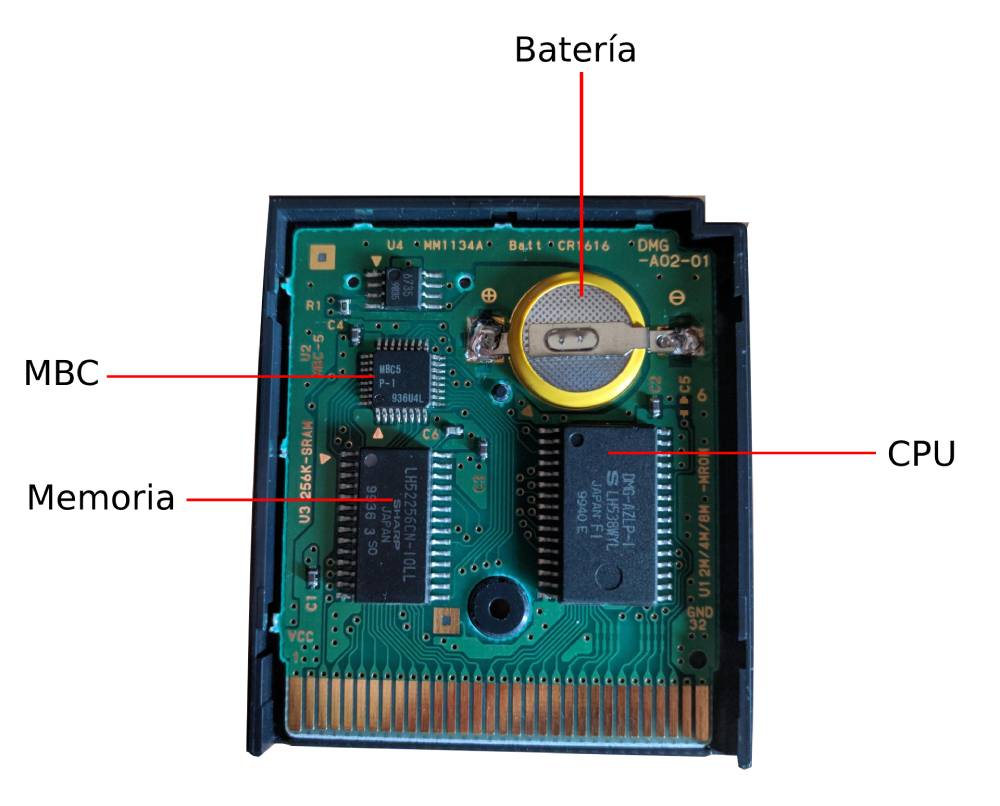
\includegraphics[width=0.7\textwidth]{include/images/cart.jpg}
    \caption{Diagrama - Cartucho de Game Boy MBC5}
    \label{figure:cart_gameboy}
\end{figure}

\subsection{No MBC: 0x00} Los juegos pequeños, que tienen un tamaño de ROM de hasta 32 KiB, no necesitan un utilizar bancos de memoria. En su lugar, la ROM se coloca directamente en la memoria en el rango de direcciones 0x0000-0x7FFF. Además, si se requiere RAM adicional (hasta 8 KiB), se puede conectar en el rango 0xA000-0xBFFF utilizando un circuito lógico.

\begin{figure}[H]
    \centering
    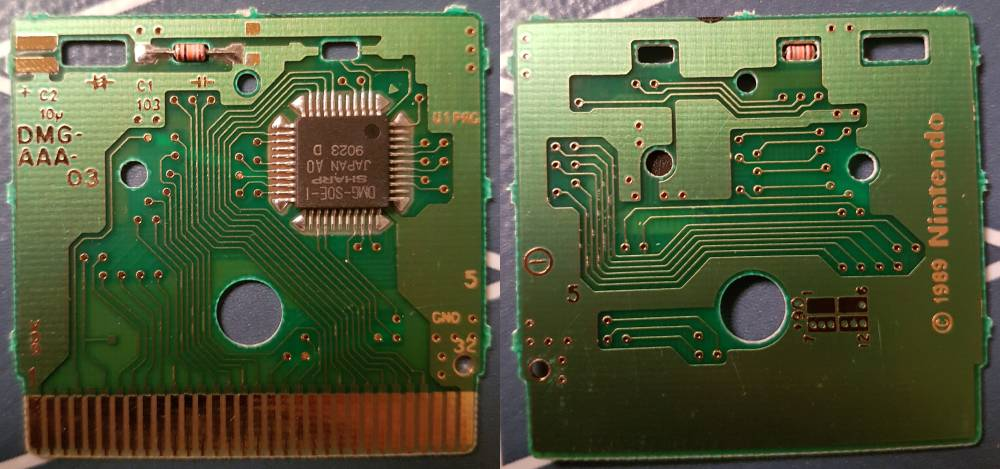
\includegraphics[width=0.6\textwidth]{include/images/nombc.jpg}
    \caption{PCB sin MBC (\cite{hardwaredatabase})}
    \label{figure:cart_no_mbc}
\end{figure}

\subsection{MBC1: 0x01-0x03} Es el modelo de chip más antiguo. Pese a ello, trabaja de forma muy similar a los más recientes, lo que facilitó la actualización de los juegos o la posibilidad de hacerlos retro-compatibles.
\\\\
En la configuración predeterminada (valor 0x00) el MBC1 soporta hasta 512KiB de ROM y un total de 32KiB de RAM mediante el uso de bancos. Esta configuración puede cambiar, por ejemplo para utilizar la parte de RAM como ROM, aumentando esta última hasta 2MiBs. Es importante tener en cuenta que la memoria en el rango de direcciones 0x0000–0x7FFF se usa tanto para leer desde la ROM como para escribir en los registros de control del MBC.

\begin{figure}[H]
    \centering
    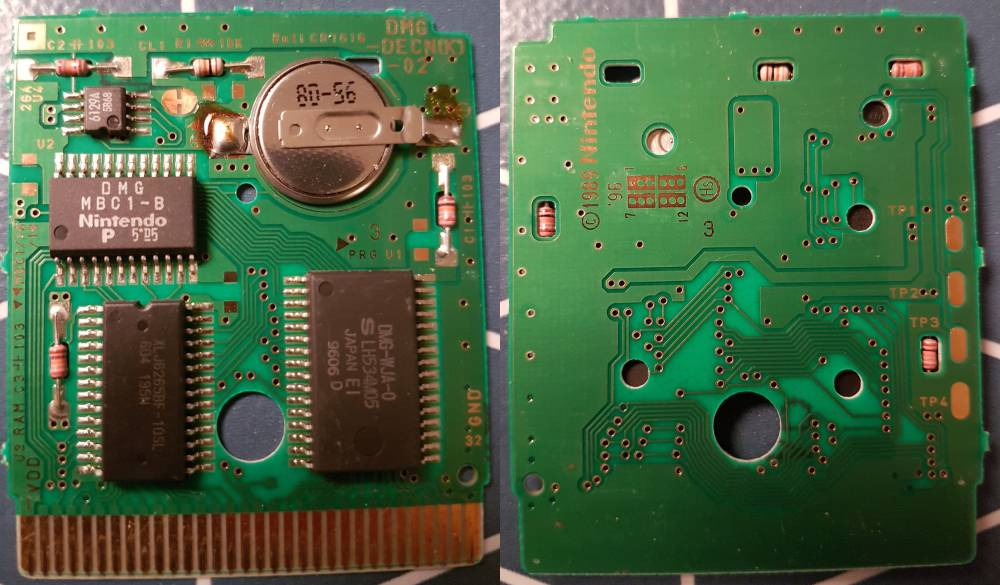
\includegraphics[width=0.6\textwidth]{include/images/mbc1.jpg}
    \caption{PCB MBC1 (\cite{hardwaredatabase})}
    \label{figure:cart_mbc1}
\end{figure}

\subsubsection{Memoria}

\paragraph{Banco de ROM 0x00: 0x0000-0x3FFF}
\label{par:rom0bank}
Esta región usualmente contiene los primeros 16KiB de ROM del cartucho (suele ser fija, es decir, no cambia).

\paragraph{Bancos de ROM 0x01-0x7F: 0x4000-0x7FFF}
Esta región puede contener cualquiera de los bancos de 16KiB posibles. La elección del banco se realiza a través del registro 0x2000-0x3FFF.

\paragraph{Banco de RAM 0x00-0x03: 0xA000-0xBFFF}
Esta región se utiliza para leer o escribir en la RAM externa presente en algunos cartuchos (generalmente de tipo 0x02 o 0x03). El acceso a esta RAM solo es posible si está activada mediante la escritura en los registros de control del MBC; de lo contrario, las lecturas devolverán un valor indefinido (comúnmente 0xFF) y las escrituras serán ignoradas.
\\\\
Los tamaños disponibles de RAM son 8 KiB (que cubre toda la región mapeada) o 32 KiB, distribuidos en 4 bancos de 8 KiB cada uno. La segunda opción solo está disponible en cartuchos con ROM de hasta 512 KiB.
\\\\
La RAM externa suele estar alimentada por una batería, lo que permite el almacenamiento de datos incluso cuando la consola está apagada. Esta batería, normalmente una celda de botón soldada en la placa del cartucho, garantiza la persistencia de los datos. Además, dado que la velocidad de la RAM externa es comparable a la RAM interna de la Game Boy, algunos desarrolladores la utilizan como memoria de trabajo adicional (WRAM), aunque esto puede limitar el espacio disponible para el almacenamiento de datos.

\subsubsection{Registros}

Las siglas ROM hacen referencia a la Read Only Memory, es decir, memoria de solo lectura. Este tipo de memoria tiene la característica de ser no modificable durante la ejecución del programa. En el caso de la Game Boy, a pesar de que algunas regiones de la memoria ROM se comportan como registros, no se puede escribir en ellas directamente. La diferencia radica en que, aunque las instrucciones pueden apuntar a estas regiones como si se tratase de registros, los valores no se almacenan físicamente en la ROM. En su lugar, la operación tiene efecto según la región designada, sin que el valor sea guardado en esa área específica de la ROM. Este comportamiento es gestionado por el controlador, que permite la alternancia entre distintas partes de la ROM en ciertos momentos durante la ejecución del juego, sin modificar el contenido original de la memoria.
\\\\
Todos estos registros tienen por defecto el valor 0x00. Para el banco de ROM será tratado como 0x01.

\paragraph{Habilitar RAM Externa: 0x0000-0x1FFF}
Para poder acceder a la RAM externa, antes debe ser activada mediante este registro. La forma de hacerlo es escribir en la región cualquier valor cuyos 4 nibbles inferiores sean el valor 0xA.
\\\\
Se recomienda a los desarrolladores dehabilitar la RAM externa una vez se haya accedido a ella, ya que si se extrae el cartucho o se apaga la consola se pueden corromper los datos.

\paragraph{Número de Banco ROM: 0x2000–0x3FFF} Este registro considera únicamente los primeros 5 bits del valor escrito, lo que implica que los valores efectivos estarán en el rango de 0x01 a 0x1F.
\\\\
En caso de que se intente escribir el valor 0x00, el sistema lo interpretará como 0x01, debido a que el \hyperref[par:rom0bank]{banco fijo de ROM} no puede ser duplicado en ambas regiones de memoria.
\\\\
Si se selecciona un número de banco mayor que el número de bancos disponibles en el cartucho, el valor del banco se ajustará (enmascarará) al número máximo permitido. Por ejemplo, en un cartucho de 256 KiB, que solo requiere 4 bits para direccionar uno de sus 16 bancos, el bit 5 será ignorado.
\\\\
En el caso de ROMs más pequeñas, que no requieren el uso completo de los 5 bits, existe una excepción que permite duplicar el banco 0 en la región 0x4000-0x7FFF. Si se escribe el valor 0x10, los primeros 4 bits indicarán la selección del banco 0, que normalmente se traduciría al banco 1. Sin embargo, dado que el bit 5 está activado, el valor completo no será interpretado como 0x00, lo que evita la traducción 00→01. Esto permite tener el banco 0 mapeado tanto en las regiones de memoria 0x0000–0x3FFF como en 0x4000–0x7FFF.
\\\\
En los casos en que la ROM es muy grande y utilice parte de la RAM para llegar a un máximo de 2MiB, se podrá llegar a utilizar un total de 128 bancos. Con 5 bits, no es posible representar todos ellos (el máximo es 0x1F). Para poder hacerlo, se deberán utilizar los dos bits del registro de la región 0x4000–0x5FFF de forma complementaria. El banco de ROM resultante se calcularía de la siguiente manera: $BancoSeleccionado = (RegistroSecundario << 5) + BancoROM$.

Por ejemplo, si se quisiese seleccionar el banco número 101, nuestro registro secundario debería tener un valor de 0x03 y el registro de ROM un 0x05:

\begin{lstlisting}[language=Consola, caption={Selección del banco de ROM en cartuchos grandes.}, label={code:bigromselectbank}]
    00000011 << 5 = 01100000 --> el valor 0x03 (0011) pasa a valer 0x60 (96 en decimal)

      0110 0000
    + 0000 0101
    ------------
      0110 0101 = 101 en decimal
\end{lstlisting}

\paragraph{Número de Banco RAM / Complementario de Banco ROM: 0x4000–0x5FFF} Registro de 2 bits que se utiliza para seleccionar el número de banco de RAM (0x00-0x03) o especificar de forma complementaria el banco de ROM. Si la ROM y la RAM no son lo suficientemente grandes, este registro no tiene ningún uso.

\paragraph{Modo de Banco: 0x6000–0x7FFF} Este registro de 1 bit controla el comportamiento del registro de 2 bit mencionado anteriormente. Los dos comportamientos pueden ser:

\begin{itemize}
    \item \textbf{0x00:} Modo por defecto. Los dos bits del registro 0x4000–0x5FFF se utilizan como bits superiores en la selección del banco de ROM. En este modo solamente se puede acceder al banco 0 de RAM. Este modo permite acceder a un tamaño máximo de 8KiB de RAM y 2MiB de ROM.
    \item \textbf{0x01:} Modo avanzado en el que las regiones 0x0000-0x3FFF y 0xA000-0xBFFF no son fijas. Los dos bits del registro 0x4000–0x5FFF se utilizan para seleccionar el banco de RAM. Esto permite un máximo de 32KiB de RAM y 512KiB de ROM. Solamente se podrán acceder a los bancos del 0x00 al 0x1F de ROM.
\end{itemize}

La forma en la que estos modos funcionan es mediante unas puertas AND que el controlador tiene entre los dos registros de selección de bancos y el segundo bit más alto de la dirección de memoria. Estas puertas en el modo 1 se deshabilitan. Un ejemplo del modo 0 a continuación:
\\\\
Supongamos que el registro de banco ROM contiene un 5, siendo la región de memoria 0x0000-0x3FFF:

\begin{lstlisting}[language=Consola, caption={Selección del banco de ROM en modo 0.}, label={code:bigromselectbankmode0}]
        00101 -> 5 en binario
    AND 00000 -> (segundo bit más alto de la dirección en la región 0x0000-0x3FFF)
    ------------
        00000 (resultado, siempre 0)
\end{lstlisting}

\textbf{Resultado:} Siempre se accede al banco 0 en esta región de memoria, sin importar el valor del registro de banco. Es por ello que esta región es "fija". Con la región de RAM 0xA000–0xBFFF pasa exactamente lo mismo, debido a que el segundo bit más alto de la dirección 0xA000 es 0.

\section{Interrupciones}

Las interrupciones son mecanismos que permiten a la CPU pausar temporalmente la ejecución del programa principal para saltar a una posición específica de memoria, conocida como vector de interrupción. Este proceso resulta útil porque puede ocurrir en cualquier parte del código, lo que facilita la respuesta a eventos externos en tiempo real.
\\\\
En la mayoría de las CPU, existe un \textit{master flag} para controlar las interrupciones, y la CPU Z80 de la Game Boy no es una excepción. Sin embargo, además de este flag, la Game Boy cuenta con registros específicos para gestionar las interrupciones. El registro maestro es el Interrupt Master Enable (IME), que se desactiva con el opcode DI, evitando que ocurra cualquier interrupción. Por el contrario, el opcode EI activa el IME, permitiendo que se procesen las interrupciones especificadas en el registro Interrupt Enable (IE, ubicado en 0xFFFF). Complementariamente, existe el registro Interrupt Flag (IF, ubicado en 0xFF0F), que marca qué interrupción en particular ha sido activada.
\\\\
Cuando ocurre una interrupción, se sigue el siguiente procedimiento:

\begin{itemize}
    \item Al activarse una interrupción, su bit correspondiente en el registro IF se establece en 1.
    \item Si tanto el IME como el bit correspondiente en el registro IE están activos, se realizan tres pasos adicionales.
    \item El IME se desactiva, evitando que otra interrupción interrumpa la que ya está en proceso.
    \item El contador de programa (Program Counter, PC) se guarda en la pila de memoria (stack).
    \item La CPU salta al vector de la interrupción correspondiente, ejecutando el código específico para manejar ese evento.
\end{itemize}
    
Este procedimiento garantiza que las interrupciones se gestionen de forma controlada, evitando conflictos y permitiendo que la CPU responda adecuadamente a eventos críticos en tiempo real.
\\\\
Cuando se producen varias solicitudes de interrupción de forma simultánea, se otorga prioridad a aquellas con un valor de bit menor. En este esquema de prioridades, el bit 0 (interrupción de VBlank) tiene la mayor prioridad, mientras que el bit 5 (interrupción del Joypad) posee la prioridad más baja.

\subsection{Tipos}

\begin{itemize}
    \item \textbf{VBlank (0x40)}: Como indica el nombre, esta interrupción se lanza cada vez que la PPU entra en el modo 1, también conocido como VBlank.
    \item \textbf{LCD STAT (0x48)}: Hay distintas maneras de que esta interrupción se active, todas ellas relacionadas con los estados del barrido de pantalla.
    \item \textbf{Timer (0x50)}: Se activa a intervalos regulares según la configuración del temporizador (TIMA).
    \item \textbf{Serial (0x58)}: Se utiliza para la comunicación serie, permitiendo que dos consolas intercambien datos a través del cable Link.
    \item \textbf{Joypad (0x60)}: Esta interrupción se activa cuando el jugador presiona un botón. Tiene ciertos inconvenientes, ya que el hardware de la consola tiene el problema del rebote de interruptor, provocando se detecten más de una vez las transiciones de los bits al pulsar un mismo botón.
\end{itemize}
\label{interrupttype}

\subsection{Registros}

\subsubsection{IME (Interrupt Master Enable)}
Se trata de un flag interno de solo escritura (no está enlazado a ninguna dirección de memoria). Controla que cualquier tipo de interrupción se pueda lanzar. Al inicio de ejecución de cualquier juego, está deshabilitada. Se maneja a través de las operaciones:
\begin{itemize}
    \item \textbf{EI}: Habilita las interrupciones (IME = 1). No toma efecto hasta la ejecución de la siguiente instrucción.
    \item \textbf{DI}: Deshabilita las interrupciones (IME = 0).
    \item \textbf{RETI}: Habilita las interrupciones y ejecuta un RET.
    \item \textbf{Cuando una interrupción está siendo procesada}: En estos momentos, para que no se solapen varias interrupciones de manera simultánea, se deshabilita (IME = 0).
\end{itemize}

\subsubsection{IE (Interrupt Enable - 0xFFFF)}
Registro de 5 bits que controla qué interrupciones \textbf{pueden} ser lanzadas:
\begin{itemize}
    \item \textbf{Bit 0}: VBlank.
    \item \textbf{Bit 1}: LCD STAT.
    \item \textbf{Bit 2}: Timer.
    \item \textbf{Bit 3}: Serial.
    \item \textbf{Bit 4}: Joypad.
\end{itemize}

\subsubsection{IF (Interrupt Flag - 0xFF0F)}
Registro de 5 bits que indica qué interrupciones \textbf{deben} ser lanzadas. Los bits se corresponden con los del IE.
Una vez la CPU maneja la interrupción, el valor del bit vuelve de manera automática a 0.

\section{Temporizadores / Timers}
\label{history_timer}
Los temporizadores son mecanismos esenciales para la sincronización y el control de eventos en el sistema. Ayudan a la CPU a gestionar y coordinar actividades en el juego, como controlar la velocidad de animaciones, gestionar el conteo de frames y mantener la precisión en la ejecución de instrucciones de tiempo crítico.

\subsection{DIV (Divisor de reloj - 0xFF04)}
Contador general de 16 bits que incrementa a una frecuencia fija de 16384Hz (incrementa cada 256 ciclos de la CPU) y aproximadamente 16779Hz en SGB. Al intentar escribir cualquier valor en el registro, se restablecen los 8 primeros bits a 0x00. En caso de que se ejecute una instrucción STOP, dejará de actualizarse hasta que se reinicie la ejecución. Solamente los 8 bits más altos (8-15) son visibles para el desarrollador, los cuales son únicamente de lectura.
\begin{table}[H]
    \centering
    \begin{tabular}{|c|c|c|}
    \hline
    \textbf{Bit} & \textbf{Incremento por ciclos de máquina} & \textbf{Incremento por ciclos de reloj} \\ \hline
    0  & 1 & 4 \\ \hline
    1  & 2 & 8 \\ \hline
    2  & 4 & 16 \\ \hline
    3  & 8  & 32 \\ \hline
    4  & 16 & 64 \\ \hline
    5  & 32 & 128 \\ \hline
    6  & 64 & 256 \\ \hline
    7  & 128 & 512 \\ \hline
    8  & 256 & 1024 \\ \hline
    9  & 512 & 2048 \\ \hline
    10 & 1024 & 4096 \\ \hline
    11 & 2048 & 8192 \\ \hline
    12 & 4096 & 16384 \\ \hline
    13 & 8192 & 32768 \\ \hline
    14 & 16384 & 65536 \\ \hline
    15 & 32768 & 131072 \\ \hline
    \end{tabular}
    \caption{Incrementos del registro DIV según ciclos de máquina y de reloj}
\end{table}

\subsection{Temporizador de contador (TIMA - 0xFF05)}
Temporizador principal que permite ejecutar acciones basadas en su cuenta. Esto es útil para activar eventos en el juego, como cambios de pantalla o actualizaciones de elementos en pantalla. Se incrementa en base a la frecuencia definida por el registro TAC (0xFF07). Cuando su valor supera 0xFF, se restrablece al valor especificado en el registro TMA (0xFF06) y se genera \hyperref[interrupttype]{su interrupción}.

\subsection{Temporizador de módulo (TMA - 0xFF06)}
Este registro almacena el valor al cual se restablece el temporizador TIMA cuando se produce un desbordamiento. Cuando TIMA llega a 0xFF y genera una interrupción, este toma el valor de TMA para continuar con el conteo.

\subsection{Controlador de temporizador (TAC - 0xFF07)}
Su bit 2 controla que el contador TIMA pueda ser incrementado (0 = Pausado, 1 = Habilitado). Los bits del 3 al 7 no tienen utilidad. Por último, con los bits 0 y 1 se puede controlar la frecuencia a la que el contador avanza:

\begin{table}[h!]
    \centering
    \resizebox{\textwidth}{!}{%
    \begin{tabular}{|c|c|c|c|c|}
    \hline
    \textbf{Selección de Reloj} & \textbf{Incremento} & \textbf{DMG, SGB2, CGB (velocidad simple)} & \textbf{SGB1} & \textbf{CGB (velocidad doble)} \\ \hline
    00 & 256 M-cycles & 4096Hz & $\sim$4194Hz & 8192Hz \\ \hline
    01 & 4 M-cycles & 262144Hz & $\sim$268400Hz & 524288Hz \\ \hline
    10 & 16 M-cycles & 65536Hz & $\sim$67110Hz & 131072Hz \\ \hline
    11 & 64 M-cycles & 16384Hz & $\sim$16780Hz & 32768Hz \\ \hline
    \end{tabular}%
    }
    \caption{Selección de modos de reloj y sus frecuencias.}
\end{table}

\subsection{Funcionamiento del Temporizador}

\begin{figure}[h]
    \centering
    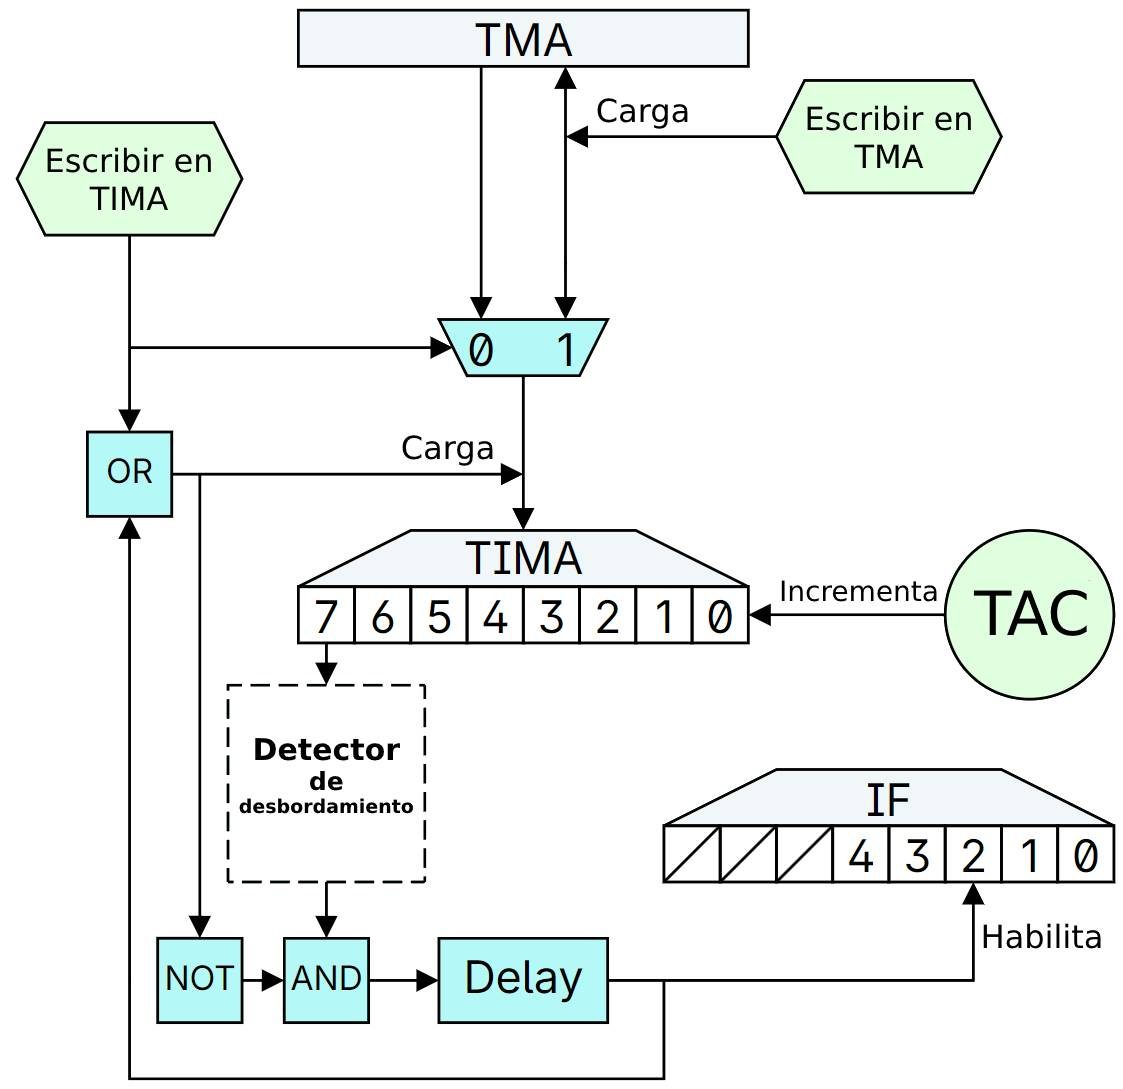
\includegraphics[width=0.7\textwidth]{include/images/tmatactima.jpg}
    \caption{Diagrama - Interacción entre TMA y TIMA (\cite{newpandocs})}
    \label{figure:tmatima}
\end{figure}

A continuación se explica el comportamiento del diagrama:

\begin{enumerate} 
    \item El temporizador TIMA se incrementa a la frecuencia especificada por el registro TAC. Cuando TIMA supera el valor 0xFF, se produce un desbordamiento, que es detectado por el sistema. 
    \item Al ocurrir un desbordamiento, se activa la interrupción correspondiente en el registro IF, y el valor de TIMA se restablece al valor presente en el registro TMA durante la señal de carga. 
    \item Si se escribe un valor en TIMA, este nuevo valor sobrescribe el actual y, además, impide que se produzca un desbordamiento en el mismo ciclo, como lo indica la operación NOT en la puerta AND. 
    \item Si se escribe un valor en TMA, TIMA tomará ese valor en el momento de un desbordamiento. 
    \item Entre TMA y TIMA se encuentra un multiplexor que controla qué valor se carga en el registro TIMA. Este multiplexor se activa al realizar una escritura en TIMA, y su funcionamiento es el siguiente: 
    \begin{itemize} 
        \item \textbf{0:} Carga el contenido de TMA en TIMA en caso de que se produzca un desbordamiento. 
        \item \textbf{1:} Permite escribir un valor directamente en TIMA desde el bus de datos de la CPU. 
    \end{itemize} 
\end{enumerate}

\section{I/O - Entrada / Salida}
Los registros pertenecientes al rango de I/O (0xFF00-0xFF70) son los siguientes:
\begin{table}[H]
    \centering
    \begin{tabular}{|c|c|c|p{5cm}|}
    \hline
    \textbf{Inicio} & \textbf{Final}   & \textbf{Primera aparición} & \textbf{Propósito} \\ \hline
    0xFF00         &                & DMG                     & Joypad \\ \hline
    0xFF01         & 0xFF02         & DMG                     & Transferencia serie \\ \hline
    0xFF04         & 0xFF07         & DMG                     & Temporizador y divisor \\ \hline
    0xFF0F         &                & DMG                     & Interrupciones \\ \hline
    0xFF10         & 0xFF26         & DMG                     & Audio \\ \hline
    0xFF30         & 0xFF3F         & DMG                     & Patrón de onda \\ \hline
    0xFF40         & 0xFF4B         & DMG                     & Control LCD, estado, posición, desplazamiento y paletas \\ \hline
    0xFF4F         &                & CGB                     & Selección de banco de VRAM \\ \hline
    0xFF50         &                & DMG                     & Activar/Desactivar el boot de ROM \\ \hline
    0xFF51         & 0xFF55         & CGB                     & VRAM DMA \\ \hline
    0xFF68         & 0xFF6B         & CGB                     & Paletas de BG / OBJ \\ \hline
    0xFF70         &                & CGB                     & Selección de banco de WRAM \\ \hline
    \end{tabular}
    \caption{Registros de I/O mapeados en memoria de la Game Boy.}
    \label{tab:memory_io_registers}
\end{table}

\subsection{Joypad: 0xFF00}

Para el control de los botones en la Game Boy, se utiliza un único registro mapeado en memoria en la dirección 0xFF00, también conocido como el registro P1. Este registro encapsula el estado de los 8 botones (A, B, Start, Select, Arriba, Abajo, Izquierda, Derecha) en un único byte, estructurado como una matriz. Cada bit representa un botón o conjunto de botones, permitiendo identificar cuál ha sido presionado.

\begin{figure}[H]
    \centering
    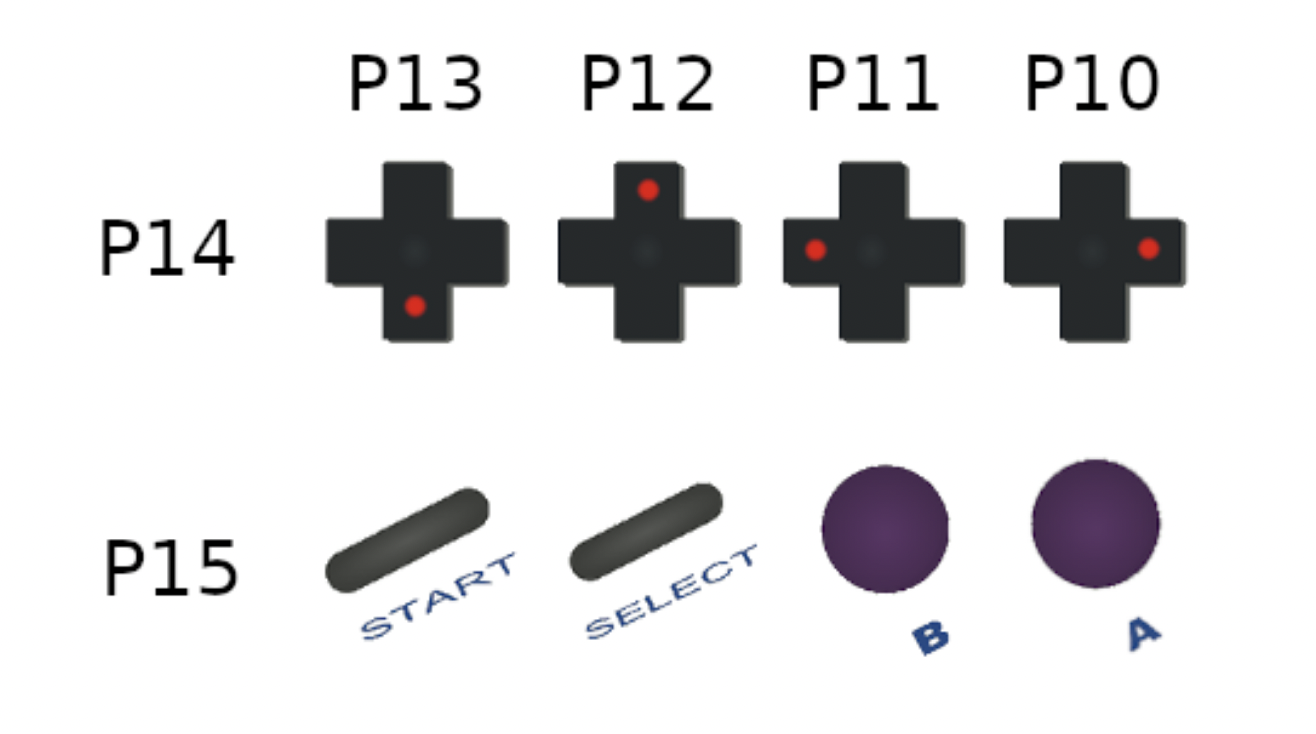
\includegraphics[width=0.7\textwidth]{include/images/joypad.png}
    \caption{Distribución del Joypad (\cite{goldensacra})}
    \label{figure:joypad}
\end{figure}

La notación P1N en las especificaciones se refiere a “Player 1” seguido del número del bit correspondiente. Por ejemplo, si se desea consultar el estado de los botones A, B, Start o Select, es necesario configurar el bit 5 en 1 y el bit 4 en 0. Esto selecciona la línea correspondiente a estos botones en la matriz virtual que el registro simula.
\\\\
Es importante destacar que el registro opera con lógica inversa: un botón presionado se representa con un valor 0, mientras que un botón sin presionar es un 1. Para trabajar de manera más intuitiva con estos valores, se puede realizar una operación complementaria, invirtiendo los bits, lo que facilita el manejo de la información en la lógica habitual (donde 1 indica botón presionado y 0 lo contrario).

\subsection{Transferencia Serie: 0xFF01-0xFF02}

Estos registros tienen relación directa con la comunicación entre dos consolas, la cual se realiza mediante un Cable Link, byte a byte. Se utiliza el protocolo SPI, en la que una de las consolas actua como "maestro" y genera una señal de reloj interna, que controla el momento exacto en que ocurre el intercambio con el resto de consolas.
\\\\
Si la consola esclava no ha cargado el siguiente byte de datos cuando comienza la transferencia, el último byte enviado será retransmitido. Por el contrario, si la consola esclava está lista para enviar un nuevo byte pero la transferencia anterior aún no ha concluido, no podrá transmitir hasta que el proceso en curso haya finalizado.

\begin{figure}[H]
    \centering
    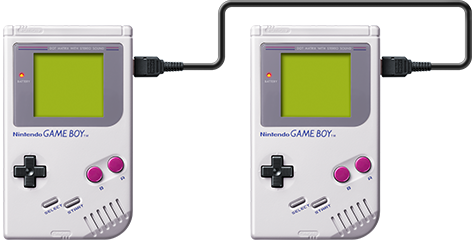
\includegraphics[width=0.6\textwidth]{include/images/link_cable.png}
    \caption{Cable Link (\cite{linkcablewiki})}
    \label{figure:linkCable}
\end{figure}

\subsubsection{SB (0xFF01): Transferencia de datos en serie}

Antes de que de comienzo la transferencia de datos, contiene el byte que va a ser enviado.
\\\\
Durante la transferencia, el registro se modifica en cada ciclo de ejecución. El bit más significativo (bit 7) es enviado, mientras que los bits restantes se desplazan a la izquierda, con el bit 6 convirtiéndose en el nuevo bit 7, siguiendo un proceso similar a un \textit{shift left}. Simultáneamente, el bit menos significativo (bit 0) se reemplaza por el bit 7 del byte que la otra consola está transfiriendo. Este procedimiento se repite durante 8 ciclos hasta completar el intercambio del byte.

\subsubsection{SC (0xFF02): Control de transmisión de datos}

\begin{table}[h!]
    \centering
    \begin{tabular}{|c|p{10cm}|}
        \hline
        \textbf{Bit} & \textbf{Descripción} \\ \hline
        7 & Indica si la transferencia de datos está en progreso o no. (0 = transferencia completa, 1 = transferencia en progreso) \\ \hline
        6 - 2 & Sin uso. \\ \hline
        1 & Solo funciona en CGB. Habilita una velocidad serial mayor (+-256kHz) \\ \hline
        0 & Selección de reloj. 0 = Reloj externo, 1 = Reloj interno de la consola maestro. \\ \hline
    \end{tabular}
    \caption{Bits del registro SC (Serial Control) de la Game Boy}
\end{table}
    

Se activa al configurar la transmisión de datos. La consola que funciona como maestro cargará un byte en el registro SB para posteriormente establecer este registro en 0x81 (0b10000001) el cual indica que se ha iniciado una transferencia y se utilizará el reloj interno de la consola maestro.
\\\\
La otra consola deberá establecer el registro en 0x80 para habilitar el puerto. Al producirse la interrupción del serial cuando la transmisión de datos finalice, establecerá el bit 7 a 0.

\paragraph{Reloj Interno}

Las velocidad del reloj interno para DMG es de 8192Hz. Esto nos da una tasa de transferencia de 1KByte por segundo. En el modo CGB, disponemos de cuatro tasas de velocidad, dependiendo del bit 1 en el registro SC, y dependiendo de si se utiliza el modo \textit{Double Speed}.

\begin{table}[h!]
    \centering
    \begin{tabular}{|c|c|c|}
        \hline
        \textbf{Frecuencia} & \textbf{Velocidad} & \textbf{Condiciones} \\ \hline
        8192Hz & 1 KB/s & Bit 1 = 0, Velocidad normal. \\ \hline
        16384Hz & 2 KB/s & Bit 1 = 0, Velocidad doble. \\ \hline
        262144Hz & 32KB/s & Bit 1 = 1, Velocidad normal \\ \hline
        524288Hz & 64KB/s & Bit 1 = 1, Velocidad doble \\ \hline
    \end{tabular}
    \caption{Frecuencias del Reloj Interno.}
\end{table}

\paragraph{Reloj Externo}

El reloj externo de forma general lo aporta la otra consola, pero si se conectara la consola a un ordenador, la frecuencia podría ser cualquiera. Hay indicios de que el modelo DMG llega a reconocer frecuencias de 500 kHz. Los pulsos de reloj no necesitan ser regulares por ambos lados, ya que la consola va a esperar pacientemente hasta recibir el siguiente bit de información.

\section{PPU}

La GPU o comunmente conocida como PPU en la Game Boy es el componente encargado de gestionar la información que se muestra por pantalla. Maneja la representación de tiles para sprites y fondos, utilizando para ello una paleta de 4 colores. La resolución de la pantalla es de 160x144 píxeles, con una tasa de refresco de 59.7Hz. Para gestionar el dibujo de cada pixel, la PPU opera en diferentes modos, conocidos como \textit{H-Blank} (Modo 0), \textit{V-Blank} (Modo 1), \textit{OAM Scan} (Modo 2) y \textit{Drawing Pixels} (Modo 3, también conocido como \textit{H-Draw}).

\begin{figure}[H]
    \centering
    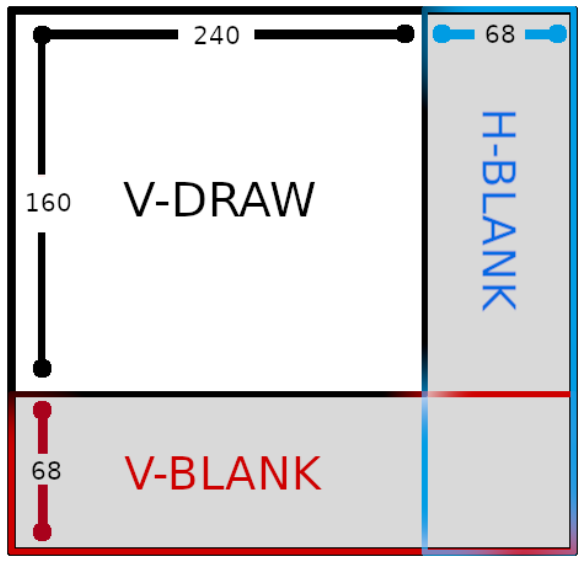
\includegraphics[width=0.4\textwidth]{include/images/ppu_modes.png}
    \caption{Modos internos de la PPU (\cite{goldensacra})}
    \label{figure:ppu_modes}
\end{figure}

\subsection{Tiles}

Los tiles son la base de la representación gráfica en la Game Boy. Cada tile tiene un tamaño de 8x8 píxeles (16 bytes en total, 2 bytes por línea) y puede ser representado por un máximo de 4 colores. De esta forma, se evita procesar los pixeles de forma individual, lo que reduce la carga de trabajo de la CPU y permite una representación más eficiente de los gráficos.
\\\\
El color de cada pixel se obtiene de un índice de 2 bits. Este índice se utiliza para acceder a la paleta de colores, que contiene un total de 4 colores. A este formato se le denomina comunmente \textbf{2BPP}, el cual hace referencia a "2 bits por pixel". La paleta de colores es compartida por todos los tiles, lo que permite una mayor eficiencia en el uso de la memoria.
\\\\ 
Para obtener el índice correcto para cada pixel, se deben leer de forma simultánea 2 líneas distintas de la memoria de tiles. La primera línea contiene los bits menos significativos, mientras que la segunda línea contiene los bits más significativos.
\\\\
Tomando como ejemplo el siguiente tile: \textit{\$3C \$7E \$42 \$42 \$42 \$42 \$42 \$42 \$7E \$5E \$7E \$0A \$7C \$56 \$38 \$7C}

\begin{figure}[H]
    \centering
    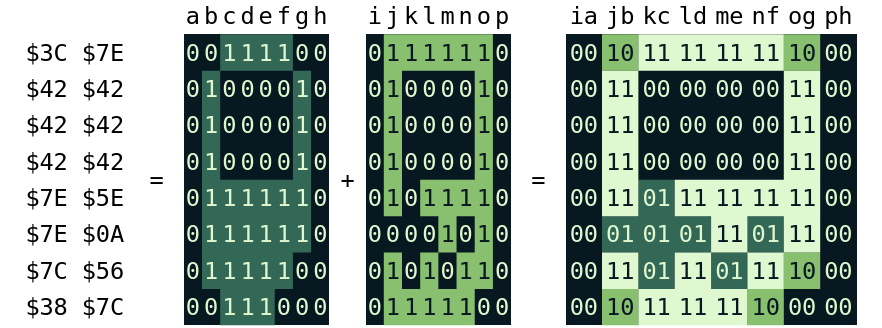
\includegraphics[width=0.8\textwidth]{include/images/colores_bits_tile.png}
    \caption{Obtención de colores para un tile (\cite{newpandocs})}
    \label{figure:tile_colors}
\end{figure}

\subsection{Capas}

La PPU de la Game Boy tiene \textbf{tres capas} diferentes: el \textbf{\textit{Background}} o Fondo principal, el \textbf{\textit{Window}} o HUD, y los \textbf{sprites}.

\begin{figure}[H]
    \centering
    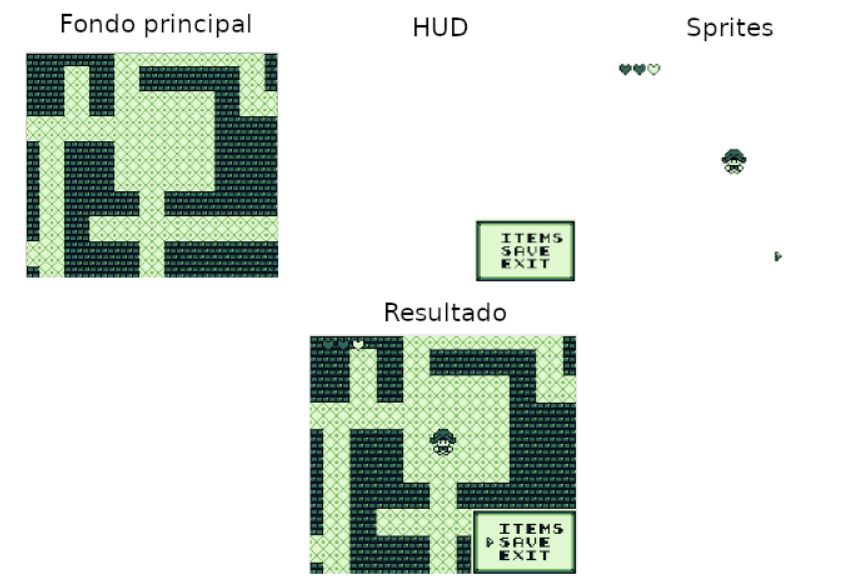
\includegraphics[width=0.8\textwidth]{include/images/layers.png}
    \caption{Capas de la PPU (\cite{goldensacra})}
    \label{figure:ppu_layers}
\end{figure}

\subsubsection{Background}

La pantalla principal es la que sirve de fondo, es decir, cualquier cosa que no vaya a necesitar actualizarse de forma constante.

\begin{figure}[H]
    \centering
    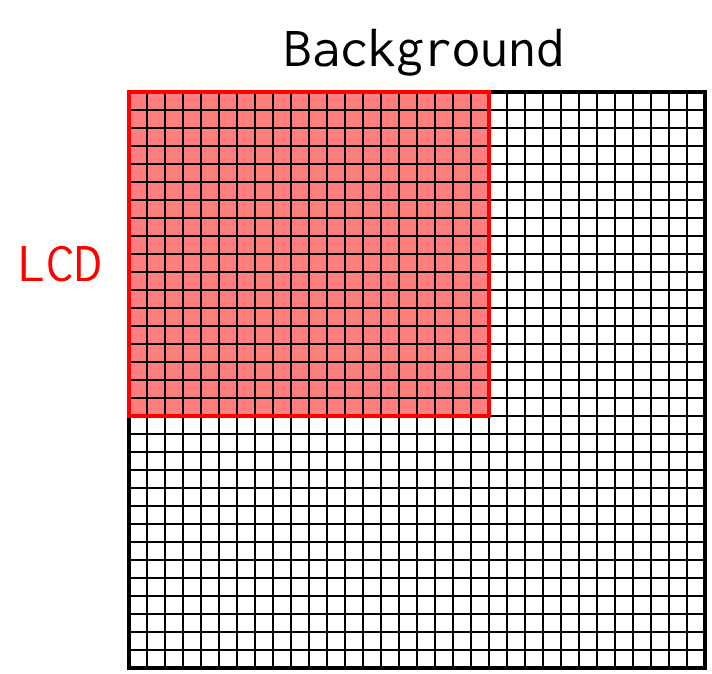
\includegraphics[width=0.4\textwidth]{include/images/grid_bg.png}
    \caption{Capa de fondo de la PPU (\cite{gbedg})}
    \label{figure:bg_layer}
\end{figure}

Está compuesto por 32x32 tiles (256x256 pixeles). De esos tiles totales, solamente una sección de 20x18 tiles (160x144 pixeles) puede ser renderizada en pantalla (\textit{LCD} en la figura previa). Esa sección se puede mover utilizando los registros SCX y SCY, las cuales establecen un offset de la posición inicial (esquina superior izquierda).

\paragraph{SCY, SCX: 0xFF42 - 0xFF43:} Estos registros definen un desplazamiento (\textit{offset}) para la posición inicial de la pantalla. Los valores pueden superar los límites inferior y derecho, pero no el superior ni el izquierdo, ya que los valores no pueden salir del rango 0-255. Si la pantalla LCD excede estos límites, la imagen se repetirá en bucle desde la posición inicial.

\begin{figure}[H]
    \centering
    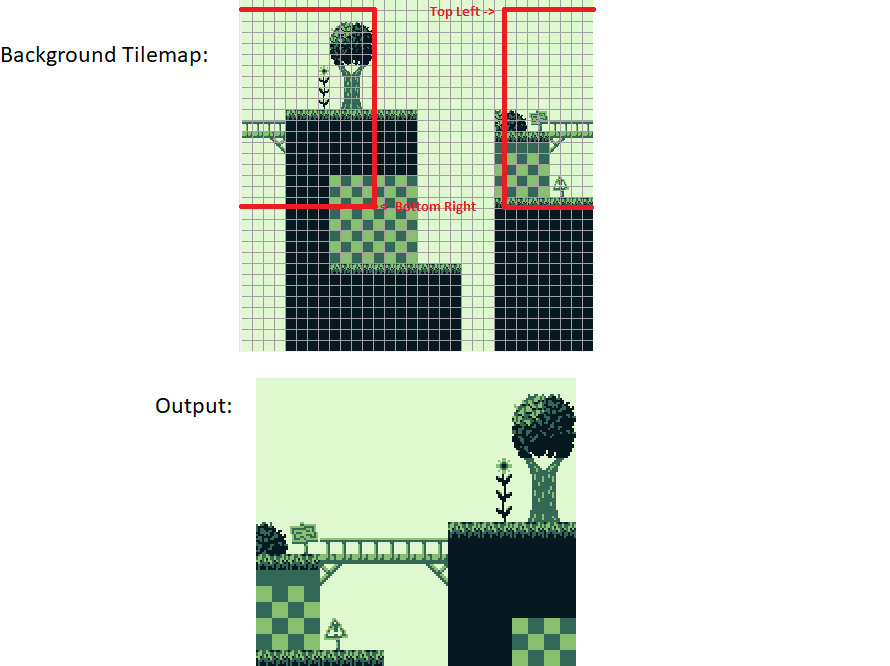
\includegraphics[width=0.8\textwidth]{include/images/scrolling_diagram.png}
    \caption{Diagrama de scroll del LCD (\cite{newpandocs})}
    \label{figure:bg_scroll}
\end{figure}

\subsubsection{Window}

Inicialmente, la ventana (Window) será invisible ya que no tendrá ninguna información a mostrar. En los videojuegos, se utiliza comúnmente para mostrar el HUD (barras de estado, menús emergentes, etc.).
\\\\
Su posición en pantalla está determinada por los registros WX y WY, donde WX incluye un desplazamiento de 7 píxeles (equivalente a un tile). Por lo tanto, si WX = 7, WY = 0, SCX = 0 y SCY = 0, la ventana se alineará exactamente sobre el Background.

\begin{figure}[H]
    \centering
    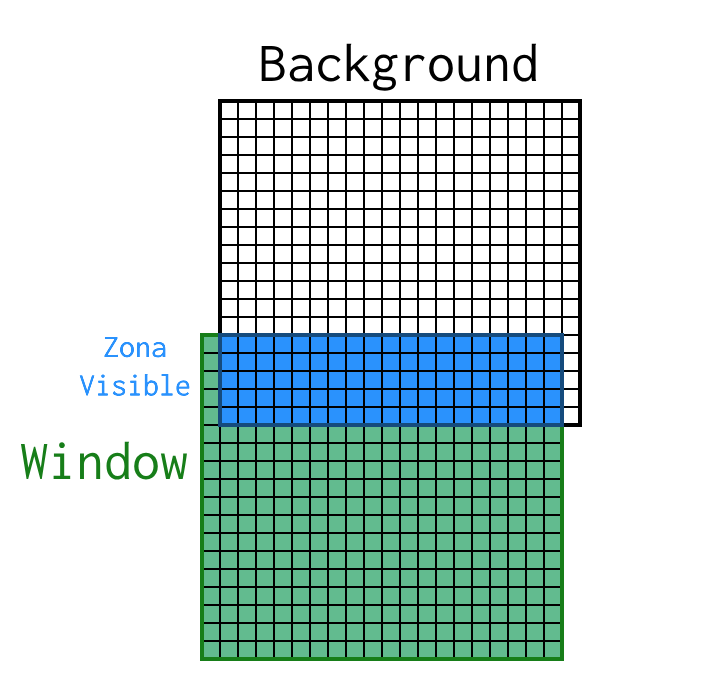
\includegraphics[width=0.4\textwidth]{include/images/grid_window.png}
    \caption{Capa de HUD de la PPU (\cite{gbedg})}
    \label{figure:window_layer}
\end{figure}

Si se analizan juegos como Pokémon Rojo/Azul, se puede apreciar mejor cómo se gestionan todas las ventanas de diálogos o de inventario.
\\\\
Por un lado, está la pantalla de Background (Screen 1), donde se carga el tilemap. Por otro lado, la ventana (Screen 2) actúa como una copia de los tiles de fondo que el scroll permite visualizar en la primera. Esto permite generar una escena completamente idéntica, de modo que, al superponer la segunda pantalla sobre la primera, no se percibe ninguna diferencia.
\\\\
La principal ventaja de este mecanismo es la posibilidad de mostrar ventanas emergentes sin necesidad de modificar el fondo ni añadir sprites, como se ilustra en la siguiente imagen.

\begin{figure}[H]
    \centering
    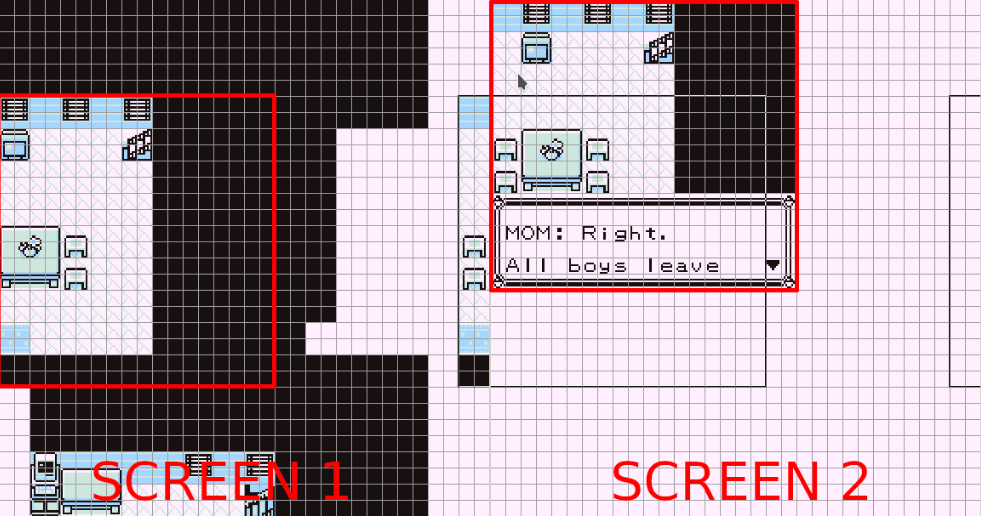
\includegraphics[width=0.8\textwidth]{include/images/window_pokemon.png}
    \caption{Dibujado de Ventanas en Pokémon Rojo/Azul (\cite{goldensacra})}
    \label{figure:window_pokemon}
\end{figure}

\paragraph{WY, WX: 0xFF4A - 0xFF4B}: Especifican el offset de la ventana respecto de la esquina superior izquierda. Los valores que pueden tomar están dentro de los siguientes rangos: 0-166 para WX y 0-143 para WY. Mencionado previamente, WX tiene un offset de 7 pixeles. 
\\\\
Hay bugs conocidos con los siguientes valores: si se establece en 0, la ventana tendrá un efecto de \textit{temblor} horizontal cuando se modifique el registro SCX. Por otro lado, si se establece en 166, la ventana se dibujará en la siguiente línea del scanline.

\subsubsection{Sprites}

Los sprites de manera general son 8x8 pixeles (2x2 tiles) que no están limitados y se mueven de forma independiente del Background y el Window. Se pueden definir también como 8x16 pixeles (2x4 tiles). La información de ellos, como se ha explicado previamente, se almacena en la memoria \hyperref[mem:oam]{OAM}.

\subsection{Registros}

A continuación se detallan los registros principales que ajustan el comportamiento y proporcionan información importante de la PPU:
\subsubsection{Control de LCD: 0xFF40}

El registro principal que controla el LCD. Permite decidir qué elementos se muestran o no por pantalla.

\begin{itemize}
    \item Bit 7: Habilita tanto la PPU como la pantalla LCD. Si se deshabilita, la pantalla se apaga y la PPU no renderiza nada. Deshabilitar la pantalla se debe hacer solamente en modo V-Blank, de otra forma puede estropear el hardware real.
    \item Bit 6: Selecciona qué tilemap va a utilizar el Window. Si está en 0, se utiliza el tilemap 0x9800-0x9BFF. Si está en 1, se utiliza el tilemap 0x9C00-0x9FFF.
    \item Bit 5: Habilita el Window. Si está en 0, el Window no se muestra. Si está en 1, el Window se muestra.
    \item Bit 4: Selecciona qué tileset va a utilizar el Background y el Window. Si está en 0, se utiliza el tileset 0x8800-0x97FF. Si está en 1, se utiliza el tileset 0x8000-0x8FFF.
    \item Bit 3: Selecciona qué tilemap va a utilizar el Background. Si está en 0, se utiliza el tilemap 0x9800-0x9BFF. Si está en 1, se utiliza el tilemap 0x9C00-0x9FFF.
    \item Bit 2: Selecciona el tamaño de los sprites. Si está en 0, los sprites son de 8x8 pixeles. Si está en 1, los sprites son de 8x16 pixeles.
    \item Bit 1: Habilita los sprites. Si está en 0, los sprites no se muestran. Si está en 1, los sprites se muestran.
    \item Bit 0: Habilita el Background y el Window. Si está en 0, el Background y el Window no se muestran. Si está en 1, el Background y el Window se muestran. En modo CGB, este bit se utiliza para habilitar el modo de prioridad de sprites.
\end{itemize}

\subsection{Modos}

Los modos de PPU definen cómo se dibujan los píxeles en pantalla. Cada uno de ellos se activa en un momento específico del ciclo de renderizado, permitiendo que la PPU realice las operaciones necesarias para mostrar la información en pantalla.

\subsubsection{Modo 0: H-Blank}



\subsubsection{Modo 1: V-Blank}
\subsubsection{Modo 2: OAM Scan}
\subsubsection{Modo 3: Drawing Pixels}


\cleardoublepage
